\documentclass[10pt, letterpaper]{article}
\usepackage[letterpaper, margin=1in]{geometry}
\usepackage{float}
\usepackage{amsmath, amssymb, amsthm}
\usepackage{newtxtext, newtxmath}
\usepackage{microtype}
\usepackage{booktabs, graphicx}
\usepackage{enumitem}
\setlist{nosep}
\usepackage[font=small, labelfont=bf, skip=4pt]{caption}
\usepackage{titlesec}
\usepackage{hyperref}
\usepackage{xcolor}
\usepackage[normalem]{ulem}

% Tracked edits (Elias): additions in red, deletions struck through in red
\DeclareRobustCommand{\eliasadds}[1]{{\color{red}#1}}
\DeclareRobustCommand{\eliasremoves}[1]{{\color{red}\sout{#1}}}

\titlespacing*{\section}{0pt}{1.2ex plus .3ex}{0.6ex plus .1ex}
\titlespacing*{\subsection}{0pt}{0.9ex plus .2ex}{0.4ex plus .1ex}
\titlespacing*{\paragraph}{0pt}{0.5ex}{1em}
\setlength{\textfloatsep}{8pt plus 2pt minus 2pt}
\setlength{\intextsep}{8pt plus 2pt minus 2pt}
\setlength{\floatsep}{8pt plus 2pt minus 2pt}
\setlength{\abovedisplayskip}{4pt plus 1pt minus 1pt}
\setlength{\belowdisplayskip}{4pt plus 1pt minus 1pt}
\setlength{\abovedisplayshortskip}{2pt}
\setlength{\belowdisplayshortskip}{2pt}
\setlength{\parskip}{0pt}

% Shorthand
\newcommand{\zco}{z^{\mathrm{coexpr}}}
\newcommand{\zex}{z^{\mathrm{expr}}}
\newcommand{\dOT}{\delta^{\mathrm{OT}}}
\newcommand{\dKL}{\delta^{\mathrm{KL}}}
\newcommand{\vKL}{\vec{\delta}^{\mathrm{KL}}}

\title{GSET: Gene Signals from Embedding Trajectories}
\author{Zeev Weizmann \and Elias Ventre}
\date{}

\begin{document}
\maketitle
\vspace{-2em}

\begin{abstract}
\noindent Mechanistic inference of gene regulatory networks from temporal transcriptomic data can become computationally prohibitive at transcriptome scale, making gene selection an important determinant of which regulatory relationships can be recovered. However, gene selection for GRN inference commonly relies on static expression or co-expression structure, rather than prioritizing dynamically informative genes whose temporal patterns capture how transcriptional programs change and relate to one another.\eliasadds{ }We introduce GSET (Gene Signals from Embedding Trajectories), an upstream retrieval framework that extracts dynamic information from temporal gene embeddings using two complementary signals: an Optimal Transport residual, which captures gene-specific deviations from global embedding movement, and a KL divergence, which detects changes in local co-expression neighborhoods. Temporal gene-embedding similarity identifies static transcriptional programs, whereas vectorial GSET signals represent coordinated temporal changes among genes, complementing this static structure. Lagged comparisons of these signals further prioritize temporal relationships between programs and candidate bridge genes associated with their transitions. Integrated with CardamomOT, GSET combines static program cores with dynamically retrieved bridge genes to construct compact, program-informed gene sets for mechanistic GRN inference, recovering regulatory structure comparably to inference over the full gene set in synthetic benchmarks. By providing a dynamic retrieval layer upstream of GRN inference, GSET links temporal transcriptional organization to compact mechanistic models that may ultimately help identify intervention points for controlling cell-state transitions.
\end{abstract}



\section{Introduction}
\label{sec:intro}

Mechanistic models of gene regulatory networks (GRNs) fitted to time-resolved single-cell data, such as CardamomOT~\cite{ventre2026cardamomot}, can recover the direction and sign of regulatory interactions, but their cost grows quickly with the number of genes, if only because the number of candidate interactions grows quadratically (Appendix~\ref{app:scalability}). Which genes enter the model therefore largely determines which regulatory relationships can be recovered. Current gene selection is largely static: genes are ranked by their variability, by membership in curated transcription-factor lists~\cite{pratapa2020beeline}, or by co-expression~\cite{langfelder2008wgcna}. The selected genes distinguish cell states~\cite{ranek2024delve}, but reveal neither how a state is actively maintained nor how cells exit it towards the next.

A cell state is held in place by coordinated gene activity~\cite{waddington1957strategy, huang2005attractor}. As noted by Kotliar et al.~\cite{kotliar2019cnmf}, ``genes act in concert to maintain a cell's identity as a specific cell type, to respond to external signals, and to carry out complex cellular activities such as replication and metabolism.'' This coordination often arises from co-regulation, with genes induced together by a shared internal or external signal~\cite{eisen1998cluster, segal2003modulenetworks}, a notion that Kotliar et al. formalised operationally as a gene expression program. Maintaining a cell state or exiting it therefore corresponds to sustaining or switching the programs that underlie it.

To represent programs, we use the structural signature that co-regulation leaves in co-expression. This signature can be captured by a co-expression graph whose nodes are genes and whose edges encode pairwise co-expression strength, for instance the soft-thresholded correlation weights of WGCNA~\cite{langfelder2008wgcna}. Graph neural networks, such as graph autoencoders~\cite{kipf2016vgae}, can then encode this graph into gene embeddings, an approach already used for gene-module and gene-interaction analysis~\cite{xing2022mlagnn, lee2022gnnwgcna}. Because such encoders place strongly co-expressed genes close together, genes of the same program form compact neighbourhoods in the latent space.

Such an embedding describes programs at a single timepoint; it does not show how they change. A program can change in two ways: its genes can shift together in activity while keeping the same co-expression partners, or a gene can acquire new partners without any change in its own expression level. With time-resolved data, genes can be embedded at every timepoint, so that each gene traces a trajectory in latent space that can reveal both kinds of change. Not every movement is informative, however: the whole embedding can drift between timepoints because of population-level responses or technical effects. Separating a gene's own movement from this global drift is analogous to decomposing an asset's return into a market component and an idiosyncratic component~\cite{sharpe1963simplified}.

A second difficulty concerns how changes in different programs relate to one another. Regulation that \emph{maintains} a program and regulation that drives \emph{exit} from it are expected to appear as co-change and as temporal precedence, respectively, but which signature a given relationship produces depends on the sampling interval relative to its biological delay, and sampling grids are rarely matched to these timescales.

\eliasadds{Because the selected genes are only an input to a downstream mechanistic model, the requirements on selection differ from those of a stand-alone analysis. First, it must scale to the whole transcriptome, since its purpose is to avoid running the mechanistic model at that scale. Second, programs must be identified \emph{consistently}, across seeds and queries; which of two genes with near-identical dynamics represents a program matters little, since either carries the same information. Third, the costs of errors are asymmetric: a spurious bridge gene only enlarges the gene budget of the downstream model, whereas a missed bridge removes a regulatory link between programs that no downstream inference can recover. Selection should therefore favour recall of bridges over precision.}

GSET (Gene \eliasremoves{Signal}\eliasadds{Signals} from Embedding Trajectories) addresses these difficulties in turn. It follows each gene along two embedding trajectories. A change of co-expression partners is visible in the co-expression embedding; because this change is defined by the relative neighbourhood structure rather than by absolute latent coordinates, we measure it with a symmetrised KL divergence~\cite{kullback1951information} between a gene's neighbourhood distributions at successive timepoints. This measure is invariant to translations and orthogonal transformations of the latent space. A change in activity is not visible there, because message passing and the scale invariance of correlation discard each gene's own expression level. We therefore embed each gene's marginal expression distribution separately, estimate the global drift with optimal transport (OT)~\cite{courty2017optimal, schiebinger2019optimal}, and keep each gene's residual. The vectorial forms of both signals reveal coordinated gene-level temporal change, complementing the static program structure recovered from the underlying embeddings. To cope with unknown timescales, GSET then compares these signals across several temporal lags, from co-change to precedence, rather than committing to a single lag. Around any query gene, the resulting relationships retrieve a compact, dynamically informative gene set, which is exactly what the mechanistic models above require. GSET thus acts as a retrieval layer, in the spirit of retrieval-augmented generation (RAG)~\cite{lewis2020rag}, and leaves the inference of causal edges to the downstream model.

\paragraph{Related work.} Gene program methods such as cNMF~\cite{kotliar2019cnmf} and Hotspot~\cite{detomaso2021hotspot} identify programs from static co-expression. GeneTrajectory~\cite{qu2025genetrajectory} orders genes along a trajectory using the OT-based gene--gene distance of Huizing et al.~\cite{huizing2022ot}\eliasadds{, computed between gene distributions over a single, static cell--cell kNN graph that pools all timepoints}. OTVelo~\cite{zhao2025otvelo} infers lagged gene--gene relations from OT couplings between \eliasadds{the \emph{cells} of consecutive} snapshots. DELVE~\cite{ranek2024delve} selects features that co-vary smoothly across neighbourhoods of a cell-similarity graph approximating the trajectory, without using sampling time or temporal order. None of these recover ordered temporal relationships between programs: cNMF and Hotspot omit time altogether, GeneTrajectory and OTVelo operate at the level of individual genes or gene pairs rather than programs, and DELVE substitutes trajectory similarity for measured time. GSET instead works on the measured timepoints and retrieves ordered temporal relationships between programs directly. \eliasadds{It also transports \emph{genes} rather than cells: after embedding, every OT and KL computation takes place in gene space, between one embedded point per gene and timepoint, so it does not require cell--cell couplings or gene--gene OT problems over cells.} Time-series GRN methods such as dynGENIE3~\cite{huynhthu2018dyngenie3}, SINCERITIES~\cite{papiligao2018sincerities} and CardamomOT~\cite{ventre2026cardamomot} infer edges directly but are typically run on a pre-selected gene panel. GSET is complementary to all of these: it is a selection layer that decides which genes a mechanistic method should see.


\paragraph{Contributions.}
\begin{itemize}[leftmargin=1.2em]
\item Two complementary gene-level signals of temporal change, an OT residual and a KL neighbourhood divergence, computed in dedicated embedding spaces. Controlled simulations show that they are preferentially sensitive to activity shifts and co-expression rewiring, respectively.

\item Vectorial forms of these signals encode coordinated gene-level temporal change; their similarity reveals organization among dynamically changing genes, complementing static program structure identifiable from concatenated co-expression embeddings.

\item A retrieval architecture that combines static program cores with dynamically retrieved bridge-gene candidates, yielding a compact, program-informed gene context rather than either the full transcriptome or a purely static selection.

\item A multi-lag comparison across several sampling resolutions shows that the distribution of temporal information across lags depends on sampling resolution, motivating aggregation across lags rather than reliance on a single fixed offset.

\item An integration with CardamomOT in which GSET acts as an upstream subnetwork-selection layer: mechanistic inference on compact, program-informed gene contexts is comparable to full-context inference on synthetic GRNs, complemented by \eliasremoves{validation}\eliasadds{a real-data check of lagged retrieval} on time-resolved rhabdomyosarcoma scRNA-seq.
\end{itemize}







%======================================================================
\section{Methods}
\label{sec:methods}
%======================================================================

\subsection{Overview}
\label{sec:overview}

We observe expression snapshots of $n$ genes at timepoints $t_0<\dots<t_M$, with cells unmatched across timepoints. GSET proceeds in five steps (Fig.~\ref{fig:overview}):

(i) embed every gene at every timepoint in a co-expression space and a marginal-expression space (\S\ref{sec:trajectories});

(ii) compute complementary per-gene, per-transition signals $\dKL$ and $\dOT$, capturing changes in local co-expression neighbourhoods and gene-specific expression activity, respectively (\S\ref{sec:ot}--\ref{sec:kl});

(iii) identify static program structure from similarity in concatenated co-expression embeddings, while retaining the KL and OT signals as gene-level trajectories of temporal change (\S\ref{sec:vectorial});

(iv) compare these signal trajectories across temporal offsets to score co-change and statistical precedence relationships and retrieve candidate bridge genes between programs (\S\ref{sec:bridge});

(v) combine static program cores with dynamically retrieved bridge candidates into a compact gene context for downstream mechanistic GRN inference with CardamomOT (\S\ref{sec:cardamom}).

\begin{figure}[t]
\centering
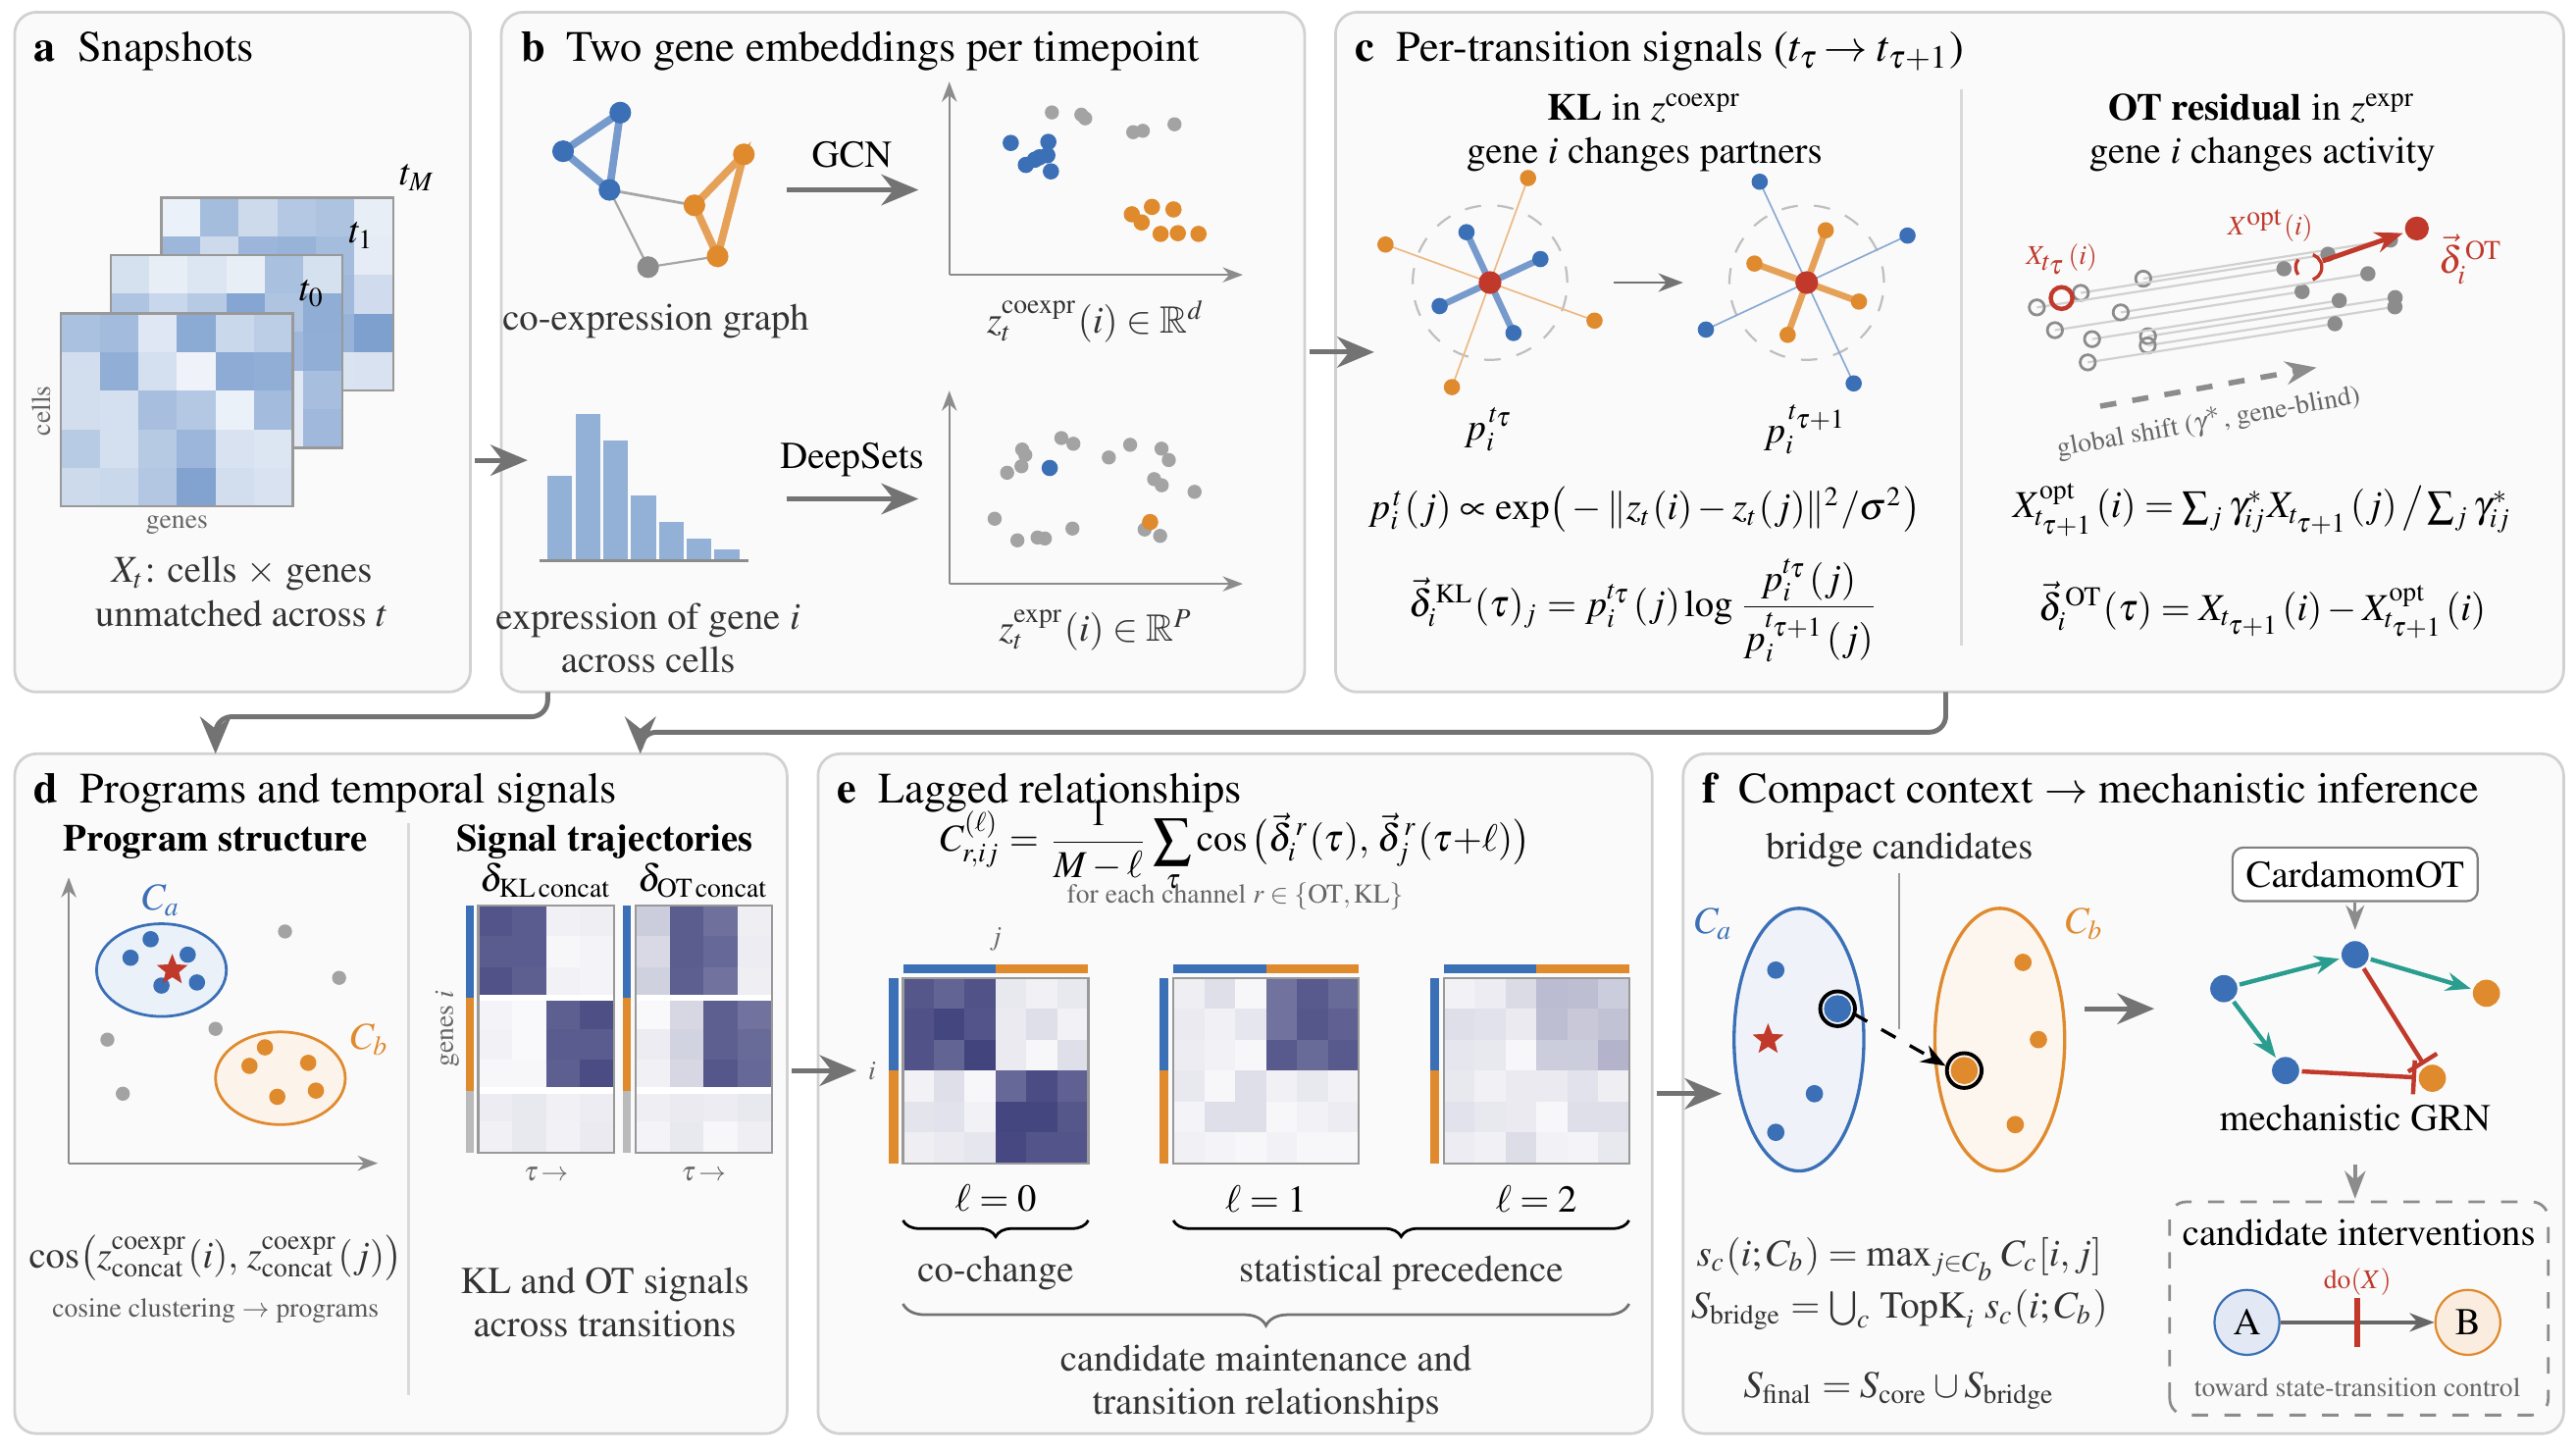
\includegraphics[width=\textwidth]{pictures/fig_overview_render_hi-1.png}
\caption{GSET overview. \textbf{(a)} Time-resolved expression snapshots, with cells unmatched across timepoints. \textbf{(b)} At each timepoint, genes are embedded in two complementary spaces: a shared-weight GCN encodes the co-expression graph into $\zco_t$, while a DeepSets encoder maps each gene's expression distribution across cells to $\zex_t$. \textbf{(c)} For each transition, $\dKL_i$ describes how gene $i$'s local neighbourhood in the co-expression embedding changes, whereas $\dOT_i$ measures its gene-specific displacement in the expression embedding after removing the gene-blind OT shift. \textbf{(d)} Similarity between concatenated co-expression embeddings defines static program structure; the KL and OT signals form gene-level trajectories across transitions. \textbf{(e)} Lagged cosine comparisons between signal trajectories quantify co-change at $\ell=0$ and statistical precedence at $\ell\geq1$, providing candidate maintenance and transition relationships across programs. \textbf{(f)} Candidate bridge genes are retrieved across lag channels and combined with static program cores into the compact context $S_{\mathrm{core}}\cup S_{\mathrm{bridge}}$. CardamomOT then performs directed, signed mechanistic GRN inference on this context, yielding candidate intervention points toward control of cell-state transitions.}
\label{fig:overview}
\end{figure}


\subsection{Gene embedding trajectories}
\label{sec:trajectories}

\paragraph{Co-expression embedding.} At each timepoint we build a WGCNA-style graph $A_t(i,j)=|\operatorname{corr}(x_i^t,x_j^t)|^{\beta}$ (with $\beta=6$) and encode it with a two-layer graph convolutional network~\cite{kipf2017gcn}. The node features are the genes' correlation profiles, and the network is trained as a graph autoencoder with an inner-product decoder~\cite{kipf2016vgae}. Its weights are shared across all timepoints, following weight tying in Siamese GNNs~\cite{krivosheev2020siamesegnn} and joint training in dynamic graph autoencoders~\cite{mahdavi2020dynvgae}. This yields $\zco_t(i)\in\mathbb{R}^d$ in which genes with similar co-expression context occupy compatible positions. Message passing averages a gene's signal with its neighbours', and correlation is scale-invariant, so this embedding discards each gene's own expression level.

\paragraph{Marginal-expression embedding.} To retain that information, a permutation-invariant DeepSets encoder~\cite{zaheer2017deep}, shared across genes and timepoints, maps gene $i$'s library-normalised expression values across the cells of timepoint $t$ to $\zex_t(i)\in\mathbb{R}^P$. The encoder uses a fixed-reference standardisation, no message passing and no information from other genes. It is trained to reconstruct the empirical quantile function of the gene's expression distribution (49 quantiles), with an additional subsample-consistency term that penalises different embeddings for two independent cell subsamples. Permutation invariance is required because cells are unmatched across timepoints and vary in number. The consistency term encourages robustness to finite-cell sampling. Full construction is given in Appendix~\ref{app:embedding}.

\paragraph{Signal-specific embedding spaces.} The OT residual measures a gene's deviation from a population-level shift, which is meaningful only if the space has a stable coordinate frame across timepoints and does not smooth over individual genes. The marginal-expression space provides both properties by construction. The co-expression space is defined only up to isometry across timepoints and is smoothed by message passing. Because the KL signal depends only on within-timepoint distances, it is well posed there. We therefore compute $\dOT$ in $\zex$ and $\dKL$ in $\zco$.

\subsection{OT residual: gene-specific deviation from the global shift}
\label{sec:ot}\label{sec:signals}

For a pair of timepoints $(s,t)$, let $X_s(i)=\zex_s(i)$ and let $\mu_s=\frac1n\sum_i\delta_{X_s(i)}$. We estimate the global shift with entropy-regularised OT, solved by Sinkhorn iterations:
\[
\gamma^\ast=\arg\min_{\gamma\in\Pi(\mu_s,\mu_t)}\ \sum_{i,j}\gamma_{ij}\,\|X_s(i)-X_t(j)\|_2^2+\varepsilon\sum_{i,j}\gamma_{ij}\log\gamma_{ij},\qquad \varepsilon=0.05 .
\]
The coupling is computed \emph{blind} to gene identities. The OT-transported position of gene $i$ is the barycentric projection $X_t^{\mathrm{opt}}(i)=\sum_j\gamma^\ast_{ij}X_t(j)/\sum_j\gamma^\ast_{ij}$, that is, the position predicted by the redistribution of the whole population. Only then do we reintroduce the gene correspondence and define
\[
\dOT_i=X_t(i)-X_t^{\mathrm{opt}}(i)\in\mathbb{R}^P,\qquad s_i^{\mathrm{OT}}=\|\dOT_i\|_2 .
\]
Unlike the raw displacement $X_t(i)-X_s(i)$, the residual separates a gene's own deviation from the collective movement. The OT plan is soft and is fitted to the population, so it can partly absorb a change that is aligned with the dominant shift, and very large coordinated programs may be partly attributed to the global trend. $\dOT$ should therefore be read as deviation from the population trend, not as total change.

\subsection{KL signal: co-expression neighbourhood reorganisation}
\label{sec:kl}

For gene $i$ at timepoint $t$, we define a distribution over the other genes from distances in $\zco_t$:
\[
p_i^t(j)=\frac{\exp\!\big(-\|\zco_t(i)-\zco_t(j)\|^2/\sigma^2\big)}{\sum_{k\neq i}\exp\!\big(-\|\zco_t(i)-\zco_t(k)\|^2/\sigma^2\big)},\qquad j\neq i,
\]
with the bandwidth $\sigma$ set independently for each transition by the median heuristic on $\zco_{t_\tau}$. The scalar signal is the symmetrised divergence $\dKL_i=D_{\mathrm{KL}}(p_i^s\|p_i^t)+D_{\mathrm{KL}}(p_i^t\|p_i^s)$. We also retain its directed per-partner contributions,
\[
\vKL_i(j)=p_i^s(j)\log\frac{p_i^s(j)}{p_i^t(j)},
\]
which record \emph{which} relationships changed. Because $p_i^t$ depends only on within-timepoint distances, $\dKL$ is invariant to translations and orthogonal transformations of either embedding. 



\subsection{Per-transition signals and program retrieval}
\label{sec:vectorial}

Applying \S\ref{sec:ot}--\eliasremoves{\S}\ref{sec:kl} to each consecutive pair $(t_\tau,t_{\tau+1})$, for $\tau=0,\dots,M-1$, gives per-transition vectors $\dOT_i(\tau)$ and $\vKL_i(\tau)$. Their concatenations over $\tau$ are $\delta_{\mathrm{OT,concat}}$ and $\delta_{\mathrm{KL,concat}}$. As reference representations without explicit differencing, we use $z_{\mathrm{global}}$, the co-expression embedding pooled over all timepoints, and $z_{\mathrm{concat}}$, the concatenation of $\zco_{t_0},\dots,\zco_{t_M}$.

Static program structure is recovered from cosine similarity in $z_{\mathrm{concat}}$, without supervision on program identity. For a query gene $q$, genes with high cosine similarity to $q$ in $z_{\mathrm{concat}}$ define its static program context. In parallel, the concatenated KL and OT signals represent each gene by its trajectory of temporal change across transitions. Cosine similarity between these vectorial signals identifies genes undergoing coordinated temporal changes, complementing the static program structure. These static and temporal representations are served interactively in Gene Program Explorer~\cite{rmsexplorer2026}.

\subsection{Lagged similarity and multi-lag bridge retrieval}
\label{sec:bridge}

For a signal $r\in\{\mathrm{OT},\mathrm{KL}\}$ and a lag $\ell\ge 0$, we define
\[
C_r^{(\ell)}[i,j]=\frac{1}{M-\ell}\sum_{\tau=0}^{M-1-\ell}\cos\!\big(\delta_i^r(\tau),\,\delta_j^r(\tau+\ell)\big).
\]
At $\ell=0$ this measures same-interval \emph{co-change} and is symmetric. For $\ell\ge1$ it measures \emph{statistical precedence}: the forward reading $C_r^{(\ell)}[i,j]$ asks whether a change in $i$ is followed $\ell$ transitions later by a similar change in $j$, whereas the reversed reading is $C_r^{(\ell)}[j,i]$. Which lag carries a temporal relationship depends on the sampling interval relative to the underlying dynamics (\S\ref{sec:precedence}). We therefore treat signal, lag, and direction combinations as complementary \emph{channels}, rather than assigning a fixed regulatory role to any single lag.

Bridge genes are retrieved independently for every ordered pair of programs $(C_a,C_b)$, so no global program ordering is required. For each channel $c$ and each gene $i\in C_a$,
\[
s_c(i;C_b)=\max_{j\in C_b}C_c[i,j],
\]
and genes in $C_b$ are scored analogously against $C_a$. The top fraction ($\mathrm{gene\_frac}$) of genes on each side is retained for each channel, and the union across channels forms the bridge context $S_{ab}$. \eliasadds{Taking the union rather than the intersection is deliberate: a false positive only enlarges the context, whereas a missed bridge cannot be recovered downstream.} Scoring genes rather than gene pairs makes the retrieval budget explicit in terms of the number of retained genes. The channel set is fixed globally and is never tuned per program pair.  In the experiments of \S\ref{sec:mechanistic}, it is $\{\mathrm{KL}^{(0)},\ \mathrm{OT}^{(0)},\ \mathrm{OT}^{(1)}\text{ forward}\}$.

Ground-truth edges are never used for ranking or selection.

\subsection{Integration with mechanistic GRN inference}
\label{sec:cardamom}

When program identities are unknown, they are discovered by clustering $z_{\mathrm{concat}}$; within each resulting cluster, program cores $S_{\mathrm{core}}$ are the top genes by within-cluster cosine centrality, combined with retrieved bridges into a fixed budget $S_{\mathrm{final}}=S_{\mathrm{core}}\cup S_{\mathrm{bridge}}$. A dedicated GRN method (here CardamomOT~\cite{ventre2026cardamomot}) is then fitted on $S_{\mathrm{final}}$. Lagged similarity can arise from shared upstream drivers as well as from direct regulation, so GSET only selects the context. Existence, direction and sign of edges are left to the mechanistic model.

%======================================================================
\section{Results}
\label{sec:results}
%======================================================================

\subsection{Datasets, baselines and evaluation protocol}
\label{sec:setup}

\paragraph{Data.}

(i) A Negative Binomial (NB) mixture with 40 genes and 5{,}000 cells per timepoint, in which co-expression rewiring and positional (marginal-expression) deviation are induced separately (Appendix~\ref{app:nb}). (ii) HARISSA~\cite{herbach2023harissa} mechanistic simulations with 100 cells per timepoint: a feedforward \emph{cascade} (C0$\to$C1$\to$C2, three ground-truth gene programs in the sense of \S\ref{sec:intro}, activated sequentially by a stimulus), a regulatory \emph{switch}, six independently generated sparse-relay cascade networks (v1--v6, 60 genes; TF--TF relay edges between consecutive programs), and a dense-relay variant (Appendix~\ref{app:random-baseline}). For the resolution sweep, the same networks are sampled on coarse, baseline and fine time grids.\eliasadds{ }(iii) A time-resolved rhabdomyosarcoma (RMS) scRNA-seq dataset~\cite{savary2023organoids} (GEO: GSE248183): six pseudotime bins ($t=0,16,\dots,80$), 13,968 cells and 8,442 genes, with cells independently annotated as quiescent, intermediate or proliferative.


\paragraph{Baselines.} $z_{\mathrm{global}}$ (static) and $z_{\mathrm{concat}}$ (trajectory of states), a lagged comparison of raw $\zco_t$ without differencing, OTVelo~\cite{zhao2025otvelo}, and the OT gene--gene distance of Huizing et al.~\cite{huizing2022ot} that underlies GeneTrajectory~\cite{qu2025genetrajectory} (``OT similarity''). We compare against GeneTrajectory's representation rather than its full pseudo-trajectory pipeline, because the pipeline answers a different question: ordering cells rather than selecting genes. Not all baselines apply to every experiment below; each subsection specifies which are compared.

\paragraph{Protocol.} Program recovery is scored by ARI, NMI and AUROC against ground-truth clusters. For edge-level precedence, true relay edges are compared with non-edges matched on both source/target program role and TF status (TF$\times$TF only). Without these two matchings, a channel could score well merely by knowing program order or TF identity. Discrimination is measured by AUROC and \emph{direction} by $P(C_{ij}>C_{ji})$ on true edges. An edge $i\to j$ is \emph{covered} by a retrieved set $S$ if $i,j\in S$. Downstream CardamomOT networks are scored by AUROC, AUPRC (chance level equal to the edge base rate) and sign agreement. Unless stated otherwise, results are averaged over three GCN/DeepSets training seeds.


\subsection{OT and KL capture complementary forms of gene-level temporal change}
\label{sec:complementarity}

On the NB-mixture dataset of \S\ref{sec:setup}, ranking genes by $\dKL$ and by $s^{\mathrm{OT}}$
reproduces the intended specialisation across two expression-level resolutions (binary: two expression levels; three-level: three on-levels plus an off-level) and across dropout rates from 0 to 0.6. KL preferentially detects co-expression rewiring and the OT residual
preferentially detects positional deviation (Appendix~\ref{app:nb},
Figs.~\ref{fig:benchmark_binary}--\ref{fig:three_modes_appendix}). The specialisation is relative rather than absolute. Under dropout, KL shows mild leakage on the positional task,
of up to about 0.7 AUROC, but stays below OT.

\subsection{Temporal signals preserve program-level organization}
\label{sec:program-recovery}

The gene-level OT and KL signals of \S\ref{sec:ot}--\ref{sec:kl} are tested for whether they retain information about program-level structure: each signal is computed independently per gene, with no access to program identity, so alignment with the known partition is evidence that the signal itself is informative rather than noise. On the HARISSA cascade scenario of \S\ref{sec:setup} (ground-truth programs C0, C1, C2), the endpoint OT residual is mutually similar within each program and dissimilar across programs, whereas the raw displacement $\zco_{T}-\zco_{0}$ in the shared co-expression embedding -- a naive geometric baseline that reflects latent movement without explicitly representing neighbourhood reorganisation -- shows no such separation (Appendix~\ref{app:vectorial}). The KL vector separates the cascade programs only through its per-transition construction $\delta_{\mathrm{KL\,concat}}$ (\S\ref{sec:vectorial}), consistent with its specialisation for co-expression rewiring (\S\ref{sec:complementarity}); the endpoint OT residual separates programs directly in both the cascade and the switch scenario of \S\ref{sec:setup} (Appendix~\ref{app:vectorial}).

Beyond this qualitative check, program recovery is quantitatively compared across representations -- including the static and trajectory baselines $z_{\mathrm{global}}$, $z_{\mathrm{concat}}$ and the literature OT-similarity baseline -- in Fig.~\ref{fig:harissa_benchmark} (Appendix~\ref{app:program-recovery-ablation}). Because program identity is encoded in timing in the cascade but not in the switch, $z_{\mathrm{global}}$ recovers the switch programs (ARI $0.84$), where each cluster is a stable co-expression module, but not the cascade programs (ARI $0.50$). Representations that retain timepoint structure close most of this gap in the cascade (ARI $0.81$--$0.90$). $z_{\mathrm{concat}}$ is the strongest and most consistent representation overall. $\delta_{\mathrm{KL\,concat}}$ tracks it closely, and it has a structural advantage that clustering scores do not show: each entry identifies which relationship changed and in which transition, which is what the precedence analysis below requires. $\delta_{\mathrm{OT\,concat}}$ is strong in the cascade (ARI $0.88$) but weak in the switch (ARI $0.51$). There, concatenation dilutes the single transition in which rewiring occurs, although the endpoint OT residual recovers the switch programs directly. OT similarity is competitive for partition recovery. Ablations (endpoint-only, full-context and max-rank variants) are also reported in Appendix~\ref{app:program-recovery-ablation}; none is consistently better than $\delta_{\mathrm{KL\,concat}}$ or $\delta_{\mathrm{OT\,concat}}$. Robustness of both vectorial signals to dropout is characterised in Appendix~\ref{app:vec-robust}.



\subsection{Temporal precedence and its dependence on sampling resolution}
\label{sec:precedence}

Precedence between programs -- whether one program's change reliably follows another's -- is distinct from the partition recovery of \S\ref{sec:program-recovery}, since a representation can recover which genes belong together without correctly ordering how programs relate over time. It is tested on both transitions (C0$\to$C1, C1$\to$C2) and scored along two separate axes, discrimination (AUROC) and direction ($P(C_{ij}>C_{ji})$, \S\ref{sec:setup}): a channel can discriminate without orienting edges correctly, or the reverse, and can be informative for one transition without being informative for the other.

\paragraph{Edge discrimination and direction.} On the TF-matched benchmark (the HARISSA sparse-relay networks v1--v6 of \S\ref{sec:setup}; Fig.~\ref{fig:directed}, Appendix~\ref{app:directed}), no single channel is informative for both transitions. Non-lag KL and lagged KL are consistently strong on C0$\to$C1 (AUROC 0.82--0.89 across the six networks) but unreliable on C1$\to$C2. Non-lag OT, OT lag-1 and OTVelo show the complementary pattern (0.78--0.90 on C1$\to$C2). OT at lag 1 and lag 2 and OTVelo orient every true edge correctly in every network ($P(C_{ij}>C_{ji})=1.00$), whereas the direction of KL lags is close to chance. $z_{\mathrm{global}}$ and lagged $\zco_t$ (\S\ref{sec:setup}) -- static or state-only, with no explicit representation of change -- do not cope: discrimination collapses on C1$\to$C2, and the direction of lagged $\zco_t$ is systematically \emph{inverted} on C0$\to$C1 (0.00 in all six networks). KL and OT together cover both transitions instead, each specialised to one (\S\ref{sec:complementarity}). OT similarity, although competitive for partitions, is weak and reverse-skewed for precedence.



\paragraph{The optimal lag follows sampling resolution.} If co-change and precedence are the same relationship seen at different resolutions, the lag at which relay edges are best discriminated should shift as the sampling grid is refined. This prediction is tested with the forward reading, averaged over three seeds per network (Table~\ref{tab:sweep}, Appendix~\ref{app:directed}). On the coarse grid, lag 0 wins on all six networks. On the baseline grid, lag 1 wins on three and lag 0 on three. On the fine grid, lag 2 wins on four (v1, v2, v5, v6), and lag 1 collapses. The reverse reading tells the same story: at lag 1, reverse AUROC is high on the coarse and baseline grids (0.68--0.94), where an interval longer than the biological delay makes the direction ambiguous, and drops on the fine grid (0.09--0.24). At lag 2 on the fine grid, the forward reading exceeds the reverse on three of six networks. Because the optimal lag is not known in advance on experimental data, GSET aggregates channels across lags.


\subsection{GSET as a retrieval layer for mechanistic GRN inference}
\label{sec:mechanistic}

GSET acts as a retrieval layer upstream of CardamomOT (\S\ref{sec:cardamom}): it selects a compact gene context, fixed in cost by the retrieval budget rather than by gene count, unlike full-context inference (\S\ref{sec:intro}, Appendix~\ref{app:scalability}). This is evaluated in three settings -- \emph{Controlled}, \emph{End-to-end} and \emph{All-edge} (Table~\ref{tab:cardamom-experiments}) -- detailed below.


\emph{Controlled} (true programs given, scored on relay edges; $\mathrm{gene\_frac}=0.25$, chosen because smaller values made C1$\to$C2 coverage fragile). Bridge retrieval and CardamomOT trained on the full system recover the relay edges with near-perfect confidence and fully correct sign (Table~\ref{tab:cardamom-experiments}). This coverage is only weak evidence on its own: random subsets of the same size achieve full coverage 33--40\% of the time. A stronger test on a denser sibling network (36 relay edges per transition, Appendix~\ref{app:random-baseline}) confirms GSET's retrieval is significantly better than random on C0$\to$C1, but significantly worse than random on C1$\to$C2. \eliasadds{Because missed bridges are the costly error (\S\ref{sec:intro}), this C1$\to$C2 deficit is the main weakness of the current channel set.}

\emph{End-to-end} (programs discovered from $z_{\mathrm{concat}}$: ARI 0.826; 50-gene budget with 14 bridges, scored on relay edges). CardamomOT fitted directly on the GSET context matches the model fitted on all 150 genes and evaluated on the same subnetwork (Full$\to$GSET), with perfect sign agreement (Table~\ref{tab:cardamom-experiments}).

\emph{All-edge} (scored on every true edge, not only relay edges, on the same 50-gene End-to-end context). The GSET context matches or exceeds Full$\to$GSET on every metric (Table~\ref{tab:cardamom-experiments}), read as \emph{no loss} from compression rather than as a gain.

\begin{table}[h]
\centering
\small
\caption{CardamomOT on GSET-retrieved contexts. \textit{Controlled} and \textit{End-to-end} are scored per transition on relay edges only; \textit{All-edge} is scored on every true edge within the same 50-gene subnetwork as End-to-end. GSET-context: CardamomOT trained on the retrieved genes; Full$\to$GSET: trained on the full 150-gene system, evaluated on the same retrieved genes. AUPRC chance equals the edge base rate (in brackets), so AUPRC is comparable only within a block.}
\label{tab:cardamom-experiments}
\setlength{\tabcolsep}{5pt}
\begin{tabular}{llcc}
\toprule
 & & C0$\to$C1 & C1$\to$C2 \\
\midrule
\textit{Controlled} [0.25--0.28\%] & Retrieved (of 100) & 76 & 80 \\
100-gene pool, true programs & Relay coverage & 4/4 & 4/4 \\
 & AUROC / AUPRC & 0.997 / 0.706 & 0.942 / 0.029 \\
\midrule
\textit{End-to-end} [7.4--9.5\%] & Relay coverage & 4/4 & 4/4 \\
50-gene budget, discovered programs & GSET-context AUROC / AUPRC & 0.880 / 0.612 & 1.000 / 1.000 \\
 & Full$\to$GSET AUROC / AUPRC & 1.000 / 1.000 & 0.895 / 0.660 \\
 & Sign agreement & 1.000 & 1.000 \\
\bottomrule
\end{tabular}

\vspace{0.3cm}

\begin{tabular}{lccc}
\toprule
\textit{All-edge} [8.2\%] & AUROC & AUPRC & Sign \\
50-gene budget, discovered programs (same context as End-to-end) & & & \\
\midrule
GSET-context & 0.756 & 0.453 & 0.762 \\
Full$\to$GSET & 0.714 & 0.342 & 0.728 \\
\bottomrule
\end{tabular}
\end{table}


\subsection{Lagged precedence traces cell-state progression in rhabdomyosarcoma}
\label{sec:rms}

On the RMS data (\S\ref{sec:setup}), GSET's lagged precedence signal is tested by whether increasing the lag from a quiescence-associated query gene traces the known quiescent$\to$intermediate$\to$proliferative progression. HSPA1B is used as the query gene because its expression is concentrated in quiescent cells, which dominate the early timepoints, making it a natural entry point.

Increasing the lag traces the quiescent$\to$intermediate$\to$proliferative progression for HSPA1B (Fig.~\ref{fig:umap_programs}), with lag-2 retrieval dominated by replication and mitotic machinery (GINS4, MCM10, KIF11, NDC80, SPC24/25, CEP55, BRCA1). This ordering holds in 6 of 7 training seeds (Fig.~\ref{fig:multiseed_umap}, Appendix~\ref{app:rms-validation}). MKI67, a canonical proliferation marker, shows the mirror pattern: already proliferative-dominant at the static level (static $P=0.916$), it remains proliferative-dominant at lag 2 ($P=0.955$), with only a transient shift toward the intermediate compartment at lag 1 ($I=0.747$; Appendix~\ref{app:rms-validation}). Both queries thus confirm the predicted progression on real, unseen data, outside any synthetic benchmark.

\begin{figure}[H]
\centering
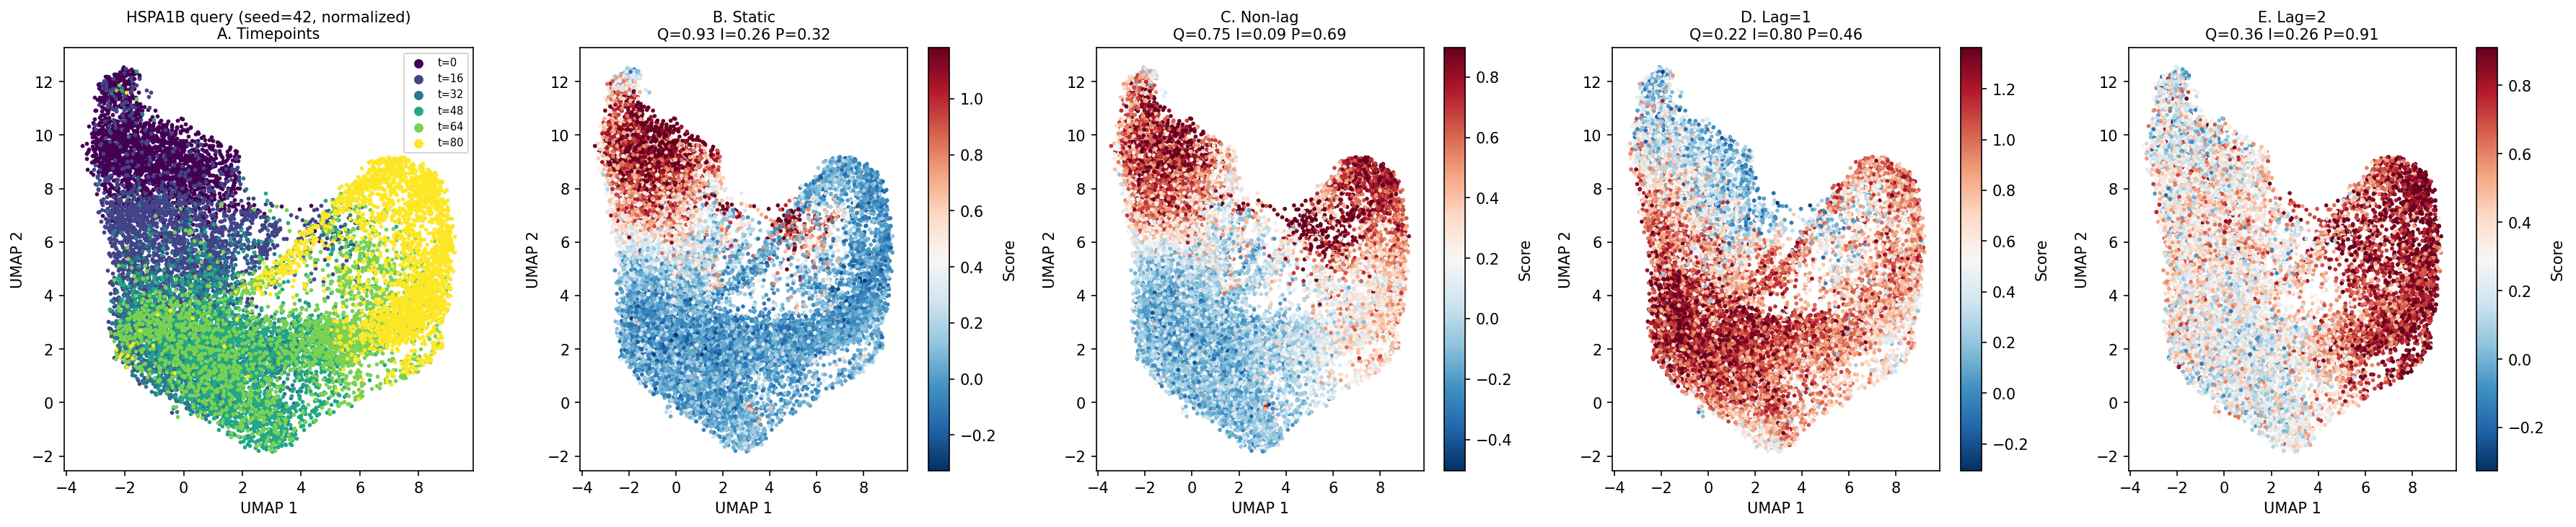
\includegraphics[width=\linewidth]{pictures/rms_normalized_seed42_HSPA1B.png}
\caption{HSPA1B query on RMS data. \textbf{A}: cells coloured by sampling time. \textbf{B}: static program (AUROC 0.925 for quiescent cells). \textbf{C}: same-interval $\delta_{\mathrm{KL}}$ retrieval (0.753, quiescent). \textbf{D}: lag 1 (0.804, intermediate). \textbf{E}: lag 2 (0.908, proliferative). Scores are Scanpy \texttt{score\_genes} on normalised log-expression, with no cell-state or sampling-time information used for retrieval; the MKI67 query is in Appendix~\ref{app:rms-validation}.}
\label{fig:umap_programs}
\end{figure}

%======================================================================
\section{Discussion}
\label{sec:discussion}
%======================================================================

GSET separates program \emph{identity} from program \emph{dynamics}. Temporal embedding similarity ($z_{\mathrm{concat}}$) is the strongest representation of which genes belong together. GSET's vectorial signals add what that representation lacks: which relationships change, and in which transition. The two signals are complementary by construction, not by scenario. KL tracks co-expression rewiring and OT tracks deviations in marginal expression, and both detect the same program when a change has both components.

The precedence experiments support two conclusions. First, program-level temporal order is not evidence of gene-level regulation. Once negatives are matched on program role and TF status, only channels that attribute a change to a specific gene and transition recover direction reliably, whereas trajectories of raw states can be consistently informative yet inverted. Second, as argued in the Introduction, the mapping from observed lag to maintenance or exit regulation depends on the sampling grid, so neither co-change nor any single positive lag is a reliable readout of regulatory role for an individual gene pair. The resolution sweep shows this migration directly. Co-change channels are also needed in their own right, because a single regulator can drive simultaneous effects across several programs rather than acting through one program to reach the next~\cite{ota2026causal}. Multi-lag aggregation is therefore a way of accommodating unknown timescales, not a tuning refinement.

\paragraph{Limitations.} Lagged similarity is not causality, and bridge genes are candidates for mechanistic inference and perturbation. Curated priors such as OmniPath~\cite{turei2021omnipath} or DoRothEA~\cite{garciaalonso2019dorothea} could filter them further. Ground-truth validation of edges, direction and sign relies on small synthetic GRNs. At an 80\% retention budget, relay coverage is only weakly informative even on the dense network (random selection covers about 64\% of edges), and the budget sensitivity of the end-to-end configuration has not been characterised. 
Finally, the directed and signed regulatory networks inferred from GSET-retrieved contexts may suggest candidate intervention points for altering cell-state transitions. This should be interpreted as a downstream perspective rather than as an intervention capability established here. A computationally supported bridge is not necessarily an effective intervention point; perturbation of predicted bridges in experimental systems will be required to establish causal control of cell-state transitions.

\paragraph{Code availability.} Code and Gene Program Explorer: \url{https://rmsexplorer.org}; source code: \url{github}.

\bibliographystyle{plain}
\bibliography{references}

\newpage
\appendix
\section{Negative Binomial mixture simulation: design and extended benchmark}
\label{app:nb}

This appendix details the synthetic benchmark of \S\ref{sec:complementarity}. AUROC compares signal genes with all remaining genes rather than with a matched null distribution. Under finite sampling, dropout, or coupling between expression distributions and measured correlations, the non-targeted signal therefore need not sit exactly at $0.5$. We interpret results through the relative specialisation of the two signals.

We simulate snapshots of a Negative Binomial mixture over $G=40$ genes and $C=5{,}000$ cells per timepoint, with $K=4$ latent cell populations. Counts are drawn from $\mathrm{NB}(r=2,\mu_k(g))$ with $\mu_{\mathrm{high}}=8.0$ and $\mu_{\mathrm{low}}=0.5$, using a split-cluster design:

\begin{center}
\begin{tabular}{lll}
\toprule
Population & Cells & High-expression genes \\
\midrule
$0a$ & $\tfrac{1}{4}C$ & genes $0$--$6$ \\
$0b$ & $\tfrac{1}{4}C$ & genes $7$--$13$ \\
$1$  & $\tfrac{1}{4}C$ & genes $14$--$26$ \\
$2$  & $\tfrac{1}{4}C$ & genes $27$--$39$ \\
\bottomrule
\end{tabular}
\end{center}

Populations $0a$ and $0b$ play equivalent roles but contain disjoint high-expression genes. Genes can therefore exchange co-expression partners between the two populations while keeping their own marginal expression level, which gives a controlled rewiring task with no positional change.

The co-expression embedding is a two-layer GCN on $A_{ij}=|\mathrm{cor}(i,j)|^\beta$, with $\beta=6$ and edges below $\tau=0.01$ discarded. Node features are Pearson correlation profiles, and the network is trained through an inner-product decoder, giving $\zco_t(i)\in\mathbb{R}^{16}$ with weights shared across timepoints. The marginal-expression embedding is the DeepSets encoder of \S\ref{sec:trajectories}. $\dKL$ and $s^{\mathrm{OT}}$ are computed as in \S\ref{sec:ot}--\ref{sec:kl}. Dropout is applied independently to each count with probability $p_d\in[0,0.6]$.

\paragraph{Rewiring task.} Genes $0$--$3$ are anchors and remain highly expressed in population $0a$ at both timepoints, so their marginal expression is unchanged. Genes $4$--$6$ move from $0a$ to $0b$, and genes $7$--$10$ move from $0b$ to $0a$. Each anchor therefore loses one set of partners and gains another. The four anchors are the signal genes.

\paragraph{Positional-deviation task.} Genes $14$--$21$ are multiplied by $3$ in every cell. Their on/off pattern, and hence approximately their correlation structure, is preserved while their marginal distributions shift. These eight genes are the signal set.

Performance is the AUROC for separating signal genes from all remaining genes, averaged over $10$ simulation draws per dropout level and $5$ GCN training seeds. Both scores behave non-monotonically near zero dropout. With $5{,}000$ cells and no dropout, the expression patterns are so regular that both representations are near-degenerate. A small dropout ($p_d\approx0.1$) breaks this, after which the specialisation is stable. In the positional task $\dKL$ rises mildly under dropout. We attribute this to count-dependent sampling noise that leaks the positional perturbation into the estimated correlations, not to genuine KL sensitivity to a marginal shift, and it stays below $s^{\mathrm{OT}}$ (Fig.~\ref{fig:benchmark_binary}).

\begin{figure}[h]
    \centering
    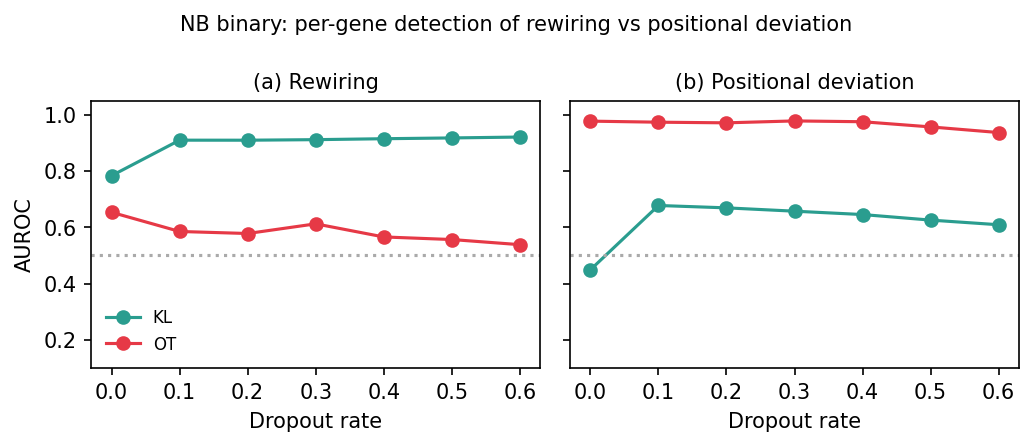
\includegraphics[width=\linewidth]{pictures/nb_binary.png}
    \caption{AUROC for detecting signal genes versus dropout in the binary NB benchmark. \textbf{(a)} Co-expression rewiring, with marginal expression held stable. \textbf{(b)} Positional deviation, with co-expression structure preserved. KL is preferentially sensitive to rewiring and the OT residual to positional deviation. Curves show seed means.}
    \label{fig:benchmark_binary}
\end{figure}

\paragraph{Three-level extension.} We replace the binary states by three on-levels, $\mu=4,10,18$, and an off-level $\mu=0.3$, keeping $0a$ and $0b$ role-equivalent. For rewiring, the anchors are the high-expression genes of the pair (genes $5$, $6$ in $0a$ and $12$, $13$ in $0b$). Genes $0$--$2$ move from $0a$ to $0b$ and genes $7$--$9$ from $0b$ to $0a$. For positional deviation, genes $14$--$21$ are multiplied by $1.5$. A factor of $3$ at these levels changes cell composition enough to perturb co-expression, so the task would no longer be approximately positional. The same specialisation holds (Fig.~\ref{fig:three_modes_appendix}). $\dKL$ detects the rewired anchors and $s^{\mathrm{OT}}$ does not. In the positional task $s^{\mathrm{OT}}$ is stronger, and $\dKL$ shows the same mild leakage, rising from chance to about $0.7$ under dropout.

\begin{figure}[h]
    \centering
    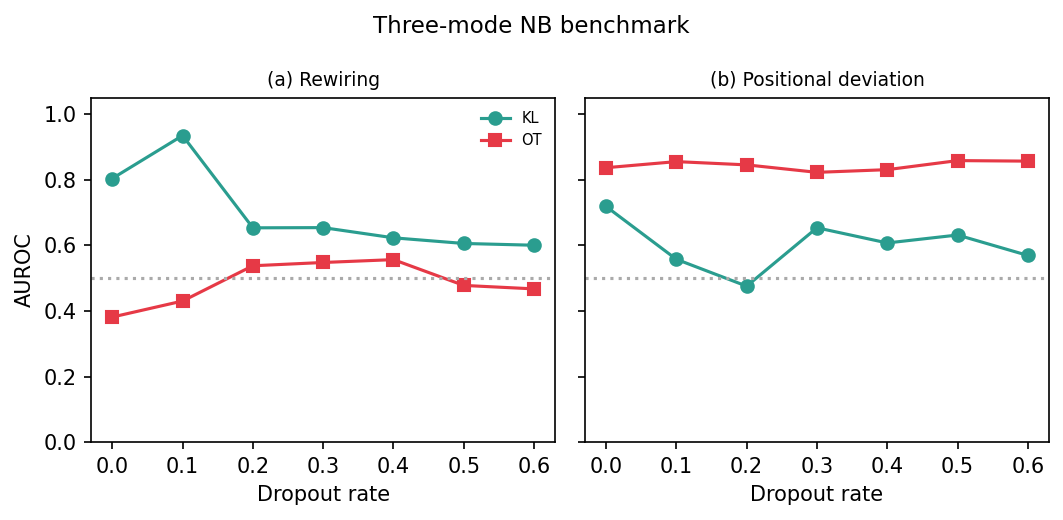
\includegraphics[width=\linewidth]{pictures/nb_three_modes.png}
    \caption{Extended three-level NB benchmark. \textbf{(a)} Rewiring: $\dKL$ detects the rewired anchors and $s^{\mathrm{OT}}$ does not. \textbf{(b)} Positional deviation: $s^{\mathrm{OT}}$ gives the stronger signal and $\dKL$ is only weakly sensitive. Curves show seed means.}
    \label{fig:three_modes_appendix}
\end{figure}

\section{Vectorial block structure in the cascade and switch scenarios}
\label{app:vectorial}

We test whether vectorial signals are organised by program on HARISSA~\cite{herbach2023harissa} simulations with known clusters. The \emph{cascade} has three clusters (C0, C1, C2) activated sequentially by a stimulus, implemented as a Negative Binomial PDMP with 24 genes. As a geometric baseline we use the direct displacement in the shared co-expression embedding, $\Delta_i^{\mathrm{GCN}}=\zco_T(i)-\zco_0(i)$. This displacement shows that a gene's latent representation moved, but its coordinates are latent GCN dimensions and do not decompose the change into contributions from specific relationships, unlike $\vKL$.

In the cascade (Fig.~\ref{fig:vectorial}), the displacement yields no clear block structure, whereas the OT residual yields three pronounced blocks aligned with the ground-truth programs. The endpoint KL vector does not recover the cascade programs: all three are active at the final timepoint, so an endpoint comparison loses the order of activation. Per-transition KL vectors retain it (\S\ref{sec:program-recovery}).

\begin{figure}[h]
    \centering
    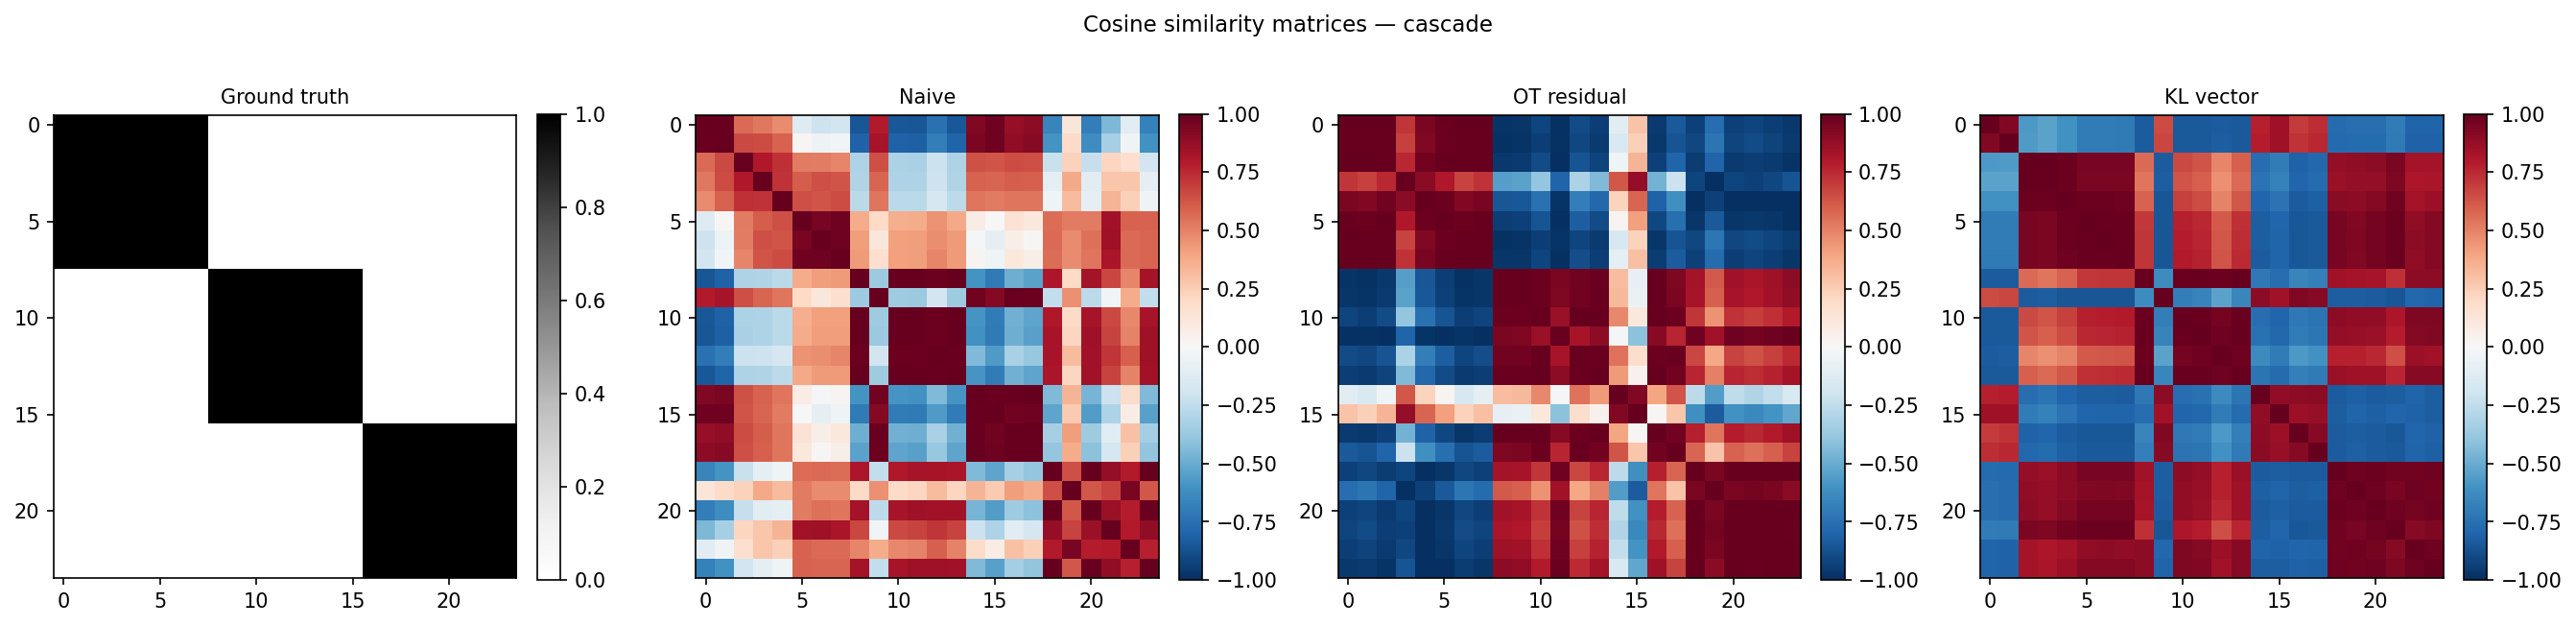
\includegraphics[width=\linewidth]{pictures/vectorial_cascade.png}
    \caption{Cosine similarity of per-gene vectors in the cascade (3 programs, 24 genes), sorted by ground-truth program. \textbf{Ground truth}: block-diagonal matrix of the true program labels, shown as a visual reference for the panels that follow. \textbf{Naive}: displacement $\zco_T-\zco_0$, with no clear blocks. \textbf{OT residual}: recovers the three programs. \textbf{KL vector}: endpoint comparison, which does not recover the sequential programs; consecutive-interval KL vectors retain the information lost here.}
    \label{fig:vectorial}
\end{figure}

In the \emph{switch} scenario, where the GRN is rewired between two conditions, both signals recover pronounced program blocks (Fig.~\ref{fig:vectorial_switch}). KL captures the coordinated reorganisation of neighbourhoods, and OT captures the accompanying coordinated change in marginal expression as one program is activated and the other suppressed. The switch therefore contains both components of program change rather than pure rewiring.

\begin{figure}[h]
    \centering
    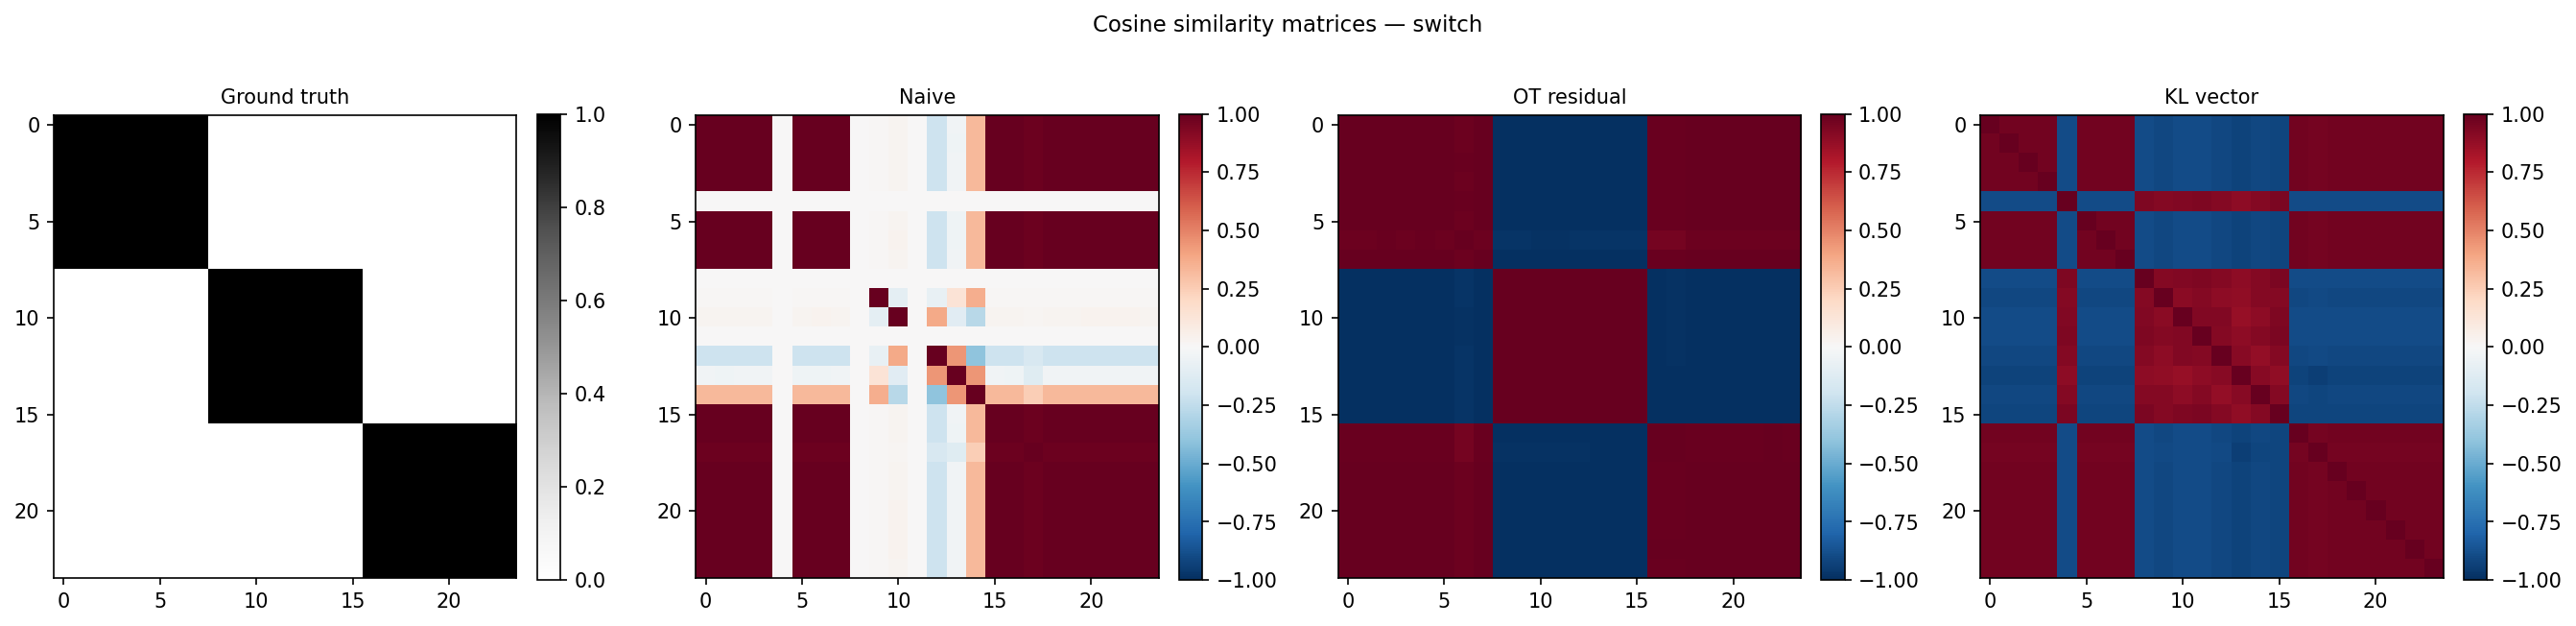
\includegraphics[width=\linewidth]{pictures/vectorial_switch.png}
    \caption{Cosine similarity of per-gene vectors in the switch scenario, sorted by ground-truth program. The leftmost panel shows the block-diagonal matrix of the true program labels as a visual reference. Both the OT residual (marginal-expression change) and the KL vector (neighbourhood reorganisation) recover the program blocks.}
    \label{fig:vectorial_switch}
\end{figure}

\section{Robustness of vectorial signals to dropout}
\label{app:vec-robust}

We vary dropout over $p_d\in[0,0.5]$ in the cascade and switch scenarios and report the gap between within-program and between-program cosine similarity. In the cascade (Fig.~\ref{fig:vectorial_dropout}), the OT gap is about $1.11$ at $p_d=0$ and about $0.91$ at $p_d=0.5$. The endpoint KL vector separates only weakly throughout (about $0.04$--$0.05$), and the naive displacement does not separate comparably. In the switch (Fig.~\ref{fig:vectorial_switch_dropout}), both signals are informative: the OT gap goes from about $1.32$ to $1.16$, and the KL gap from about $1.08$ to $0.32$. OT is thus robust in both scenarios, whereas KL is strongly informative when co-expression reorganisation is present but more sensitive to dropout. The specialisation follows the type of change encoded by each space, not the scenario.

\begin{figure}[h]
    \centering
    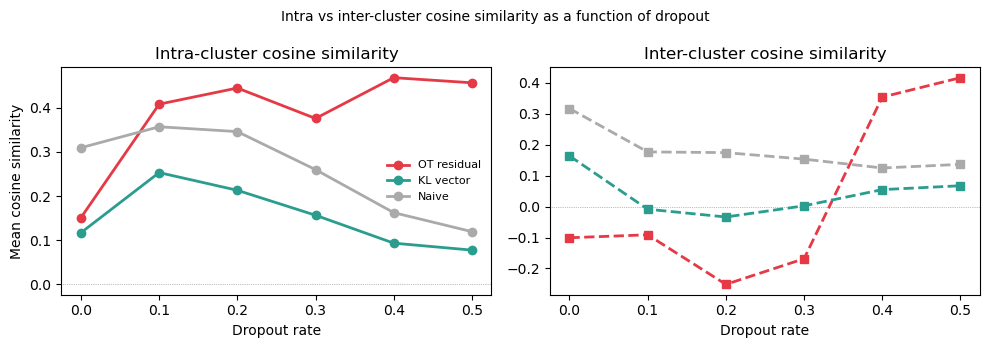
\includegraphics[width=\linewidth]{pictures/vectorial_dropout.png}
    \caption{Within- versus between-program cosine similarity versus dropout in the cascade. OT keeps strong separation; the endpoint KL vector and the naive displacement do not.}
    \label{fig:vectorial_dropout}
\end{figure}

\begin{figure}[h]
    \centering
    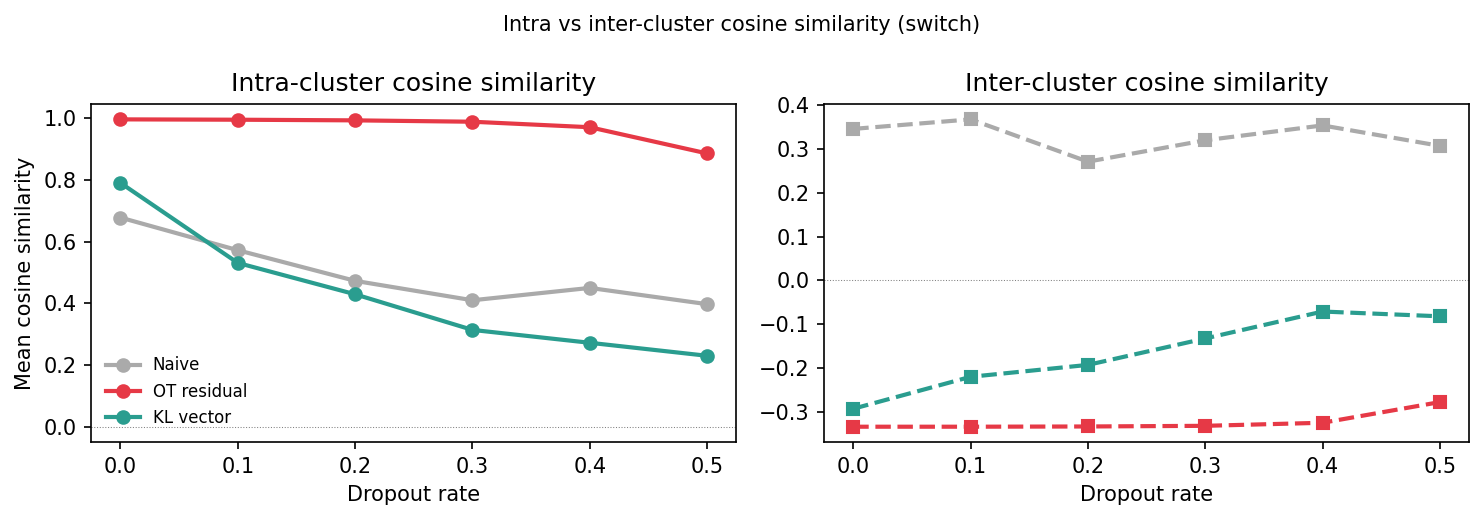
\includegraphics[width=\linewidth]{pictures/vectorial_switch_dropout.png}
    \caption{Within- versus between-program cosine similarity versus dropout in the switch. Both signals separate programs at low dropout; OT remains separated across the range, whereas KL separation decreases with dropout.}
    \label{fig:vectorial_switch_dropout}
\end{figure}

\section{Program-recovery ablation}
\label{app:program-recovery-ablation}

\begin{figure}[h]
\centering
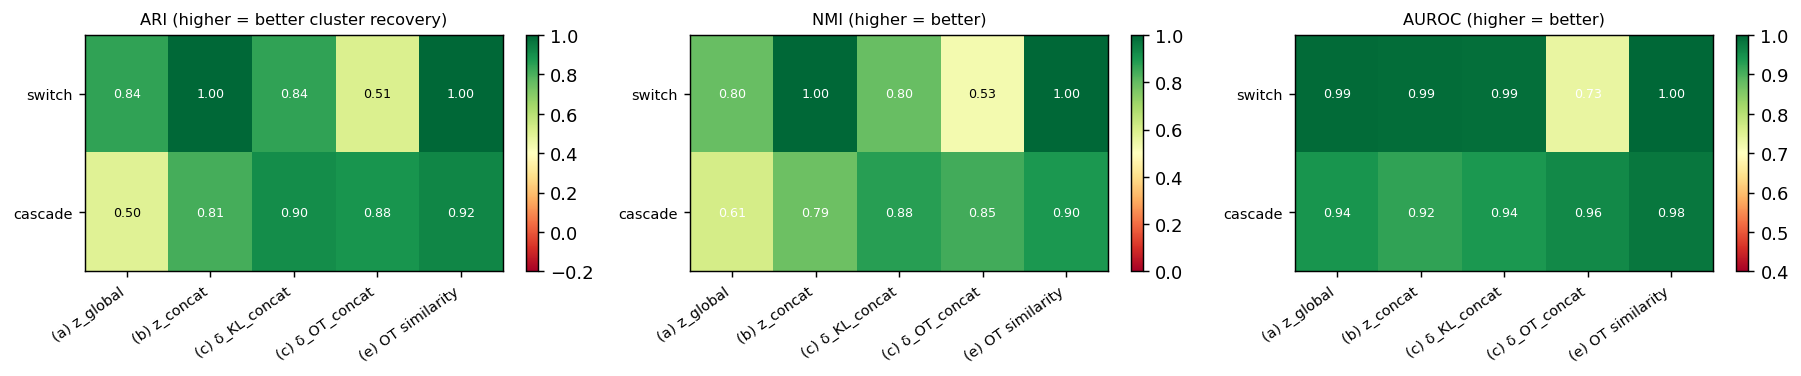
\includegraphics[width=\linewidth]{pictures/gene_programme_recovery.png}
\caption{Program recovery on HARISSA \emph{cascade} and \emph{switch} (ARI, NMI, AUROC). $z_{\mathrm{global}}$: static baseline; $z_{\mathrm{concat}}$: trajectory baseline; $\delta_{\mathrm{KL\,concat}}$, $\delta_{\mathrm{OT\,concat}}$: GSET signals; OT similarity: gene--gene distance of~\cite{huizing2022ot} underlying GeneTrajectory~\cite{qu2025genetrajectory}.}
\label{fig:harissa_benchmark}
\end{figure}

Figure~\ref{fig:harissa_benchmark_supp} reports the six variants omitted from Fig.~\ref{fig:harissa_benchmark}:
\begin{itemize}
\item the endpoint-only OT residual (there is no endpoint-only $\dKL$ variant, since resolving sequential activation requires per-transition vectors; Appendix~\ref{app:vectorial});
\item the full-context variants $\mathrm{full\_OT\_concat}$ and $\mathrm{full\_KL\_concat}$, which concatenate $z_{\mathrm{concat}}$ with $\delta_{\mathrm{OT\,concat}}$ or $\delta_{\mathrm{KL\,concat}}$;
\item three max-rank combinations: $\mathrm{MaxRank}(\mathrm{OT\text{-}OT},\mathrm{OT\,concat})$, $\mathrm{MaxRank}(\mathrm{OT},\mathrm{KL})$ and $\mathrm{MaxRank}(\mathrm{OT\text{-}OT},\mathrm{KL})$.
\end{itemize}
None is consistently better than $\delta_{\mathrm{KL\,concat}}$ or $\delta_{\mathrm{OT\,concat}}$ in either scenario.

\begin{figure}[h]
    \centering
    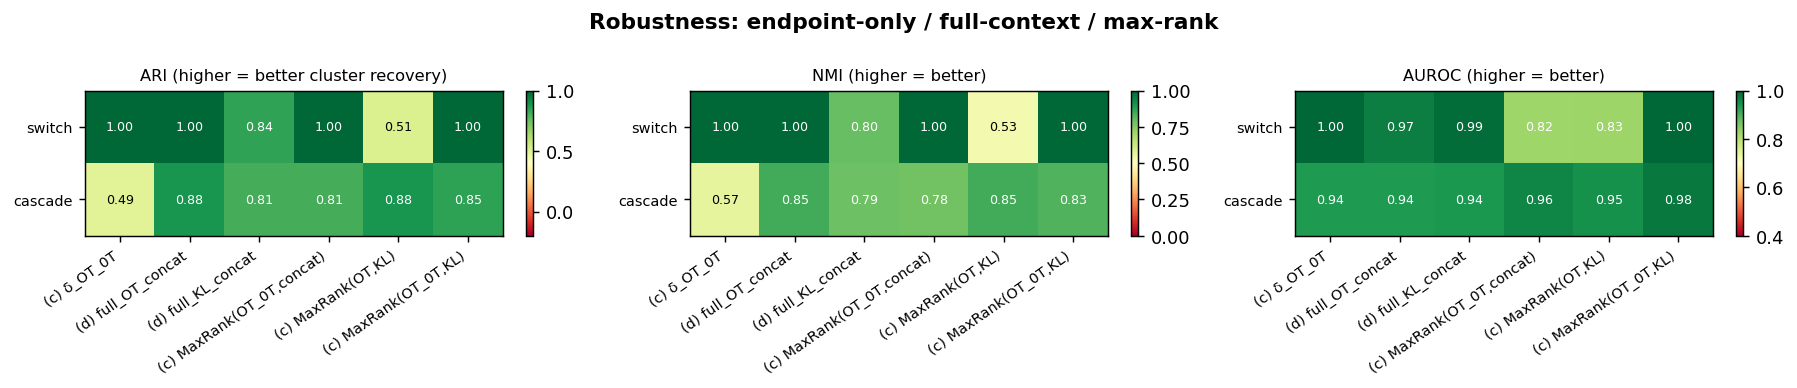
\includegraphics[width=\linewidth]{pictures/gene_programme_recovery_supplementary.png}
    \caption{Program-recovery ablation (ARI, NMI, AUROC) for the endpoint-only, full-context and max-rank variants.}
    \label{fig:harissa_benchmark_supp}
\end{figure}


\section{TF-matched relay-edge benchmark: full figure and resolution sweep}
\label{app:directed}

\begin{figure}
\centering
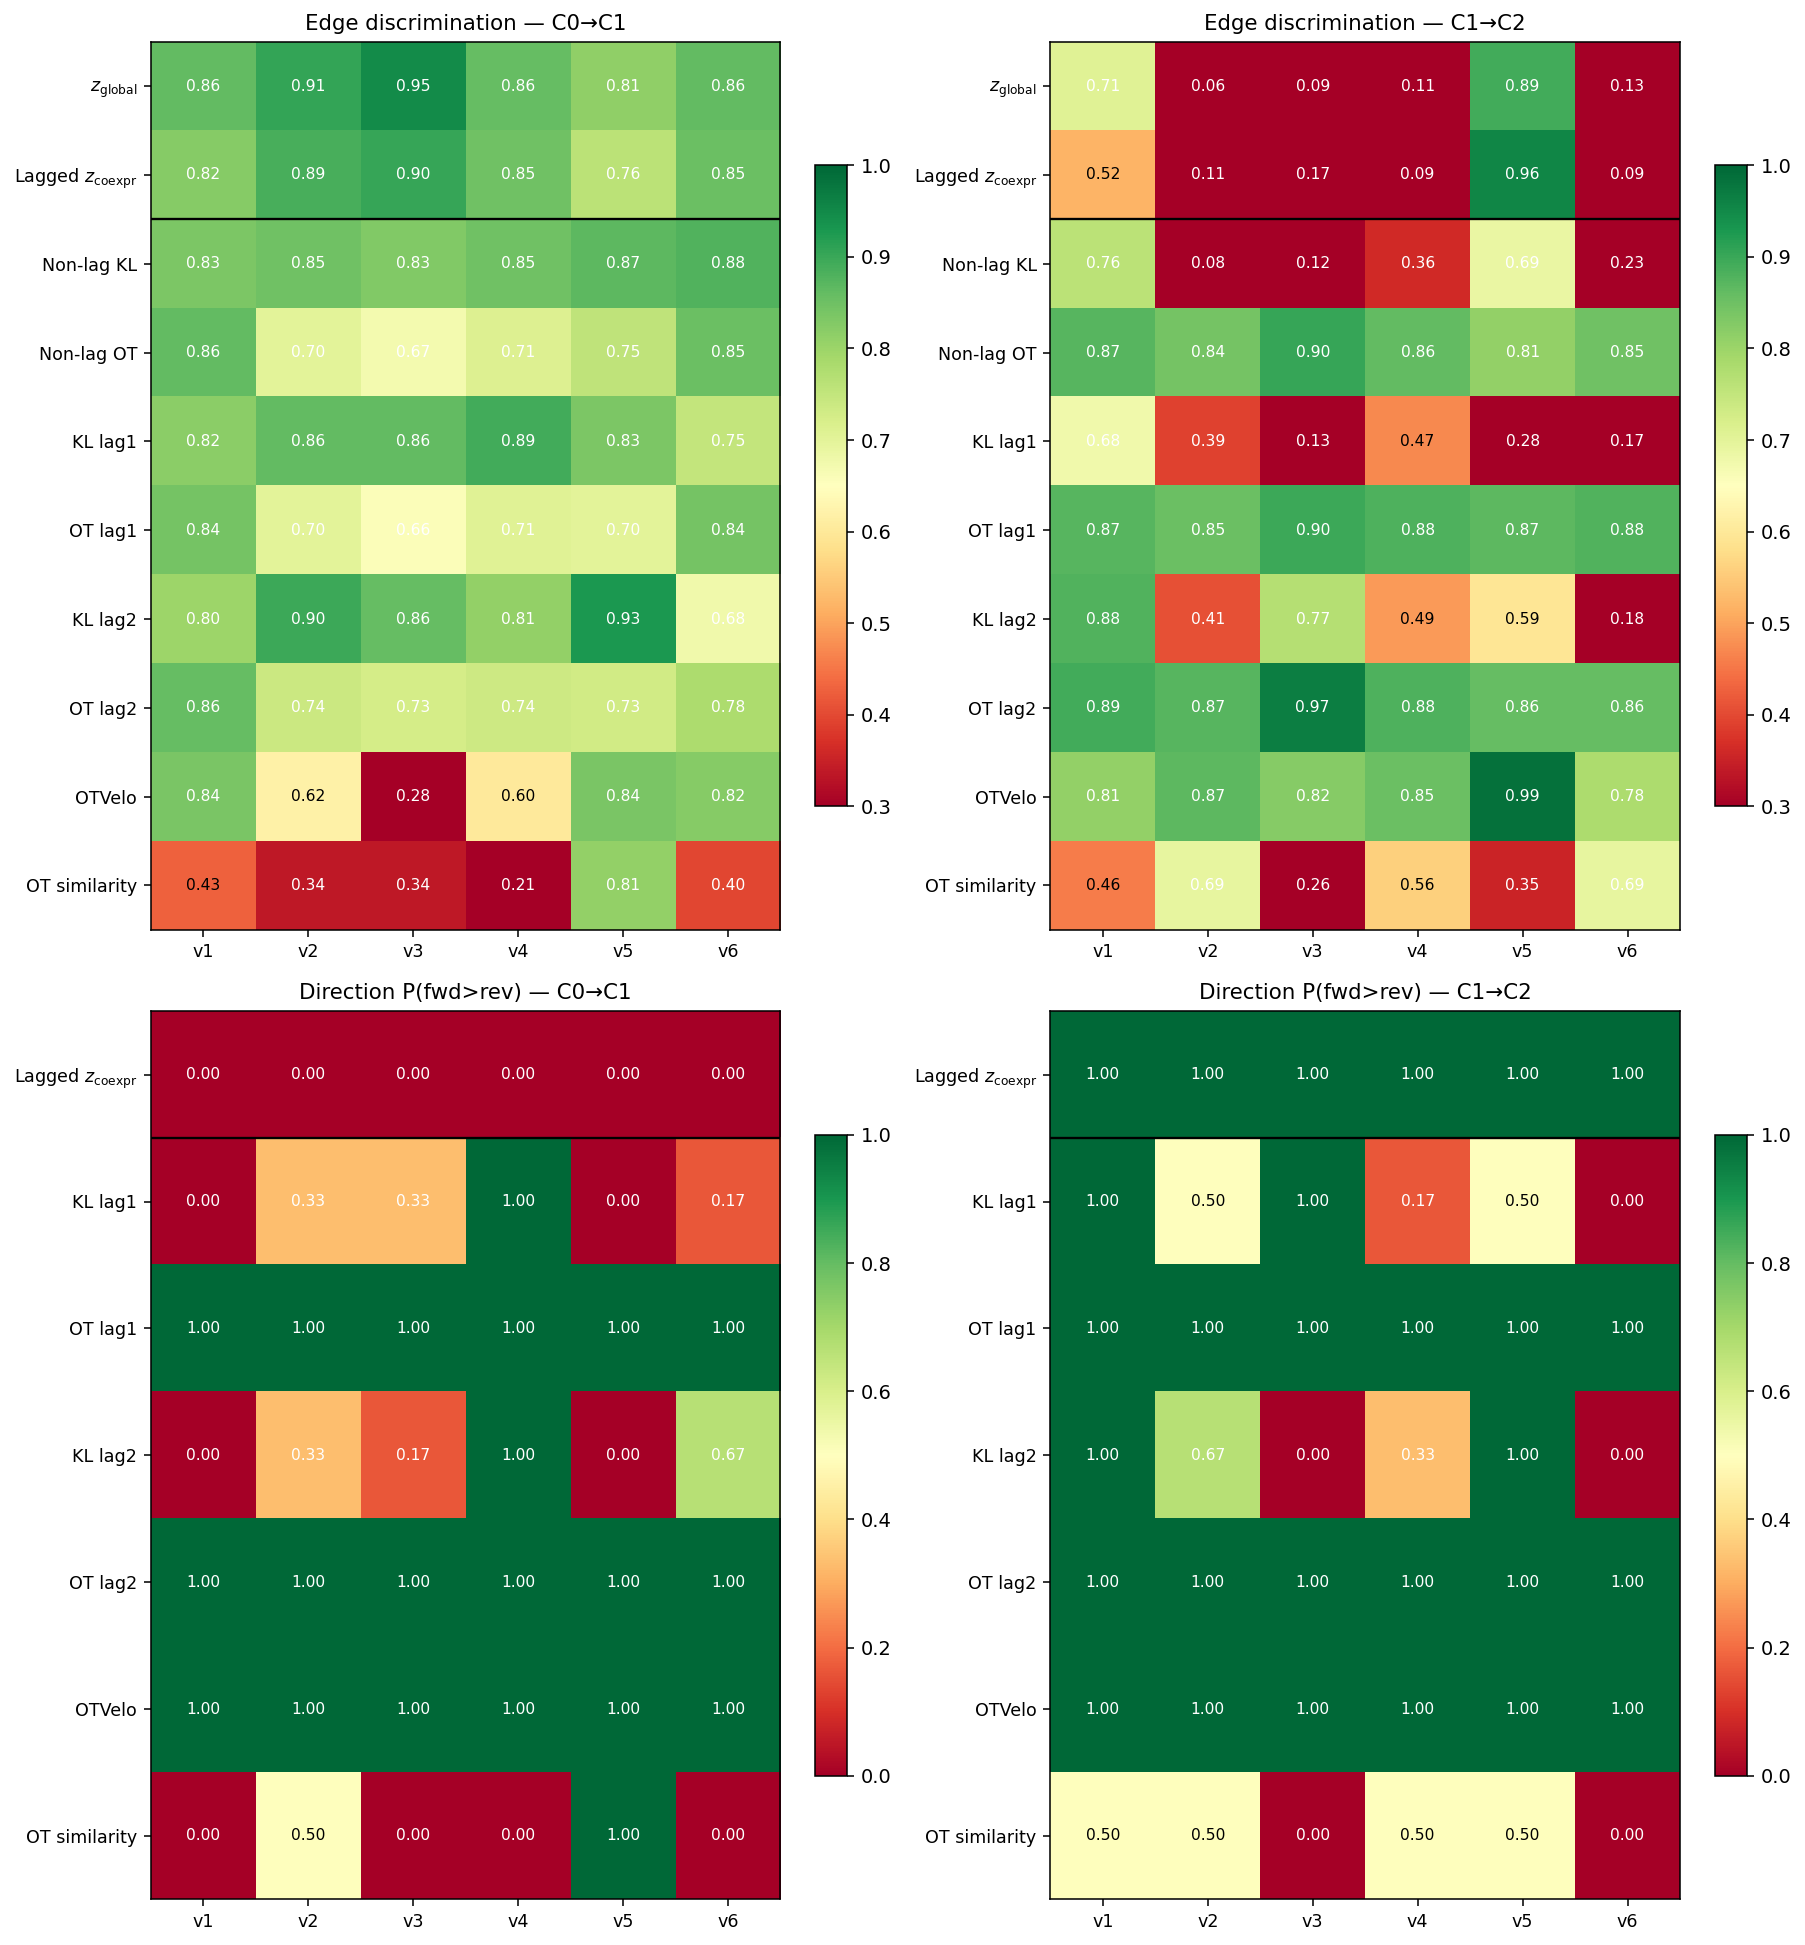
\includegraphics[width=\linewidth]{pictures/directed_benchmark_tfmatched.png}
\caption{TF-matched relay-edge benchmark on six sparse-relay networks (v1--v6), shown separately for C0$\to$C1 and C1$\to$C2. \textbf{Top}: edge-discrimination AUROC. \textbf{Bottom}: direction $P(C_{ij}>C_{ji})$ on true edges. Channels: partition controls ($z_{\mathrm{global}}$, lagged $\zco$), GSET co-change and lag-1/lag-2 channels, OTVelo and OT similarity. Chance is 0.5 in both rows; values are means over three seeds.}
\label{fig:directed}
\end{figure}

\begin{table}[H]
\centering
\small
\caption{Forward-reading edge-discrimination AUROC by sampling resolution and lag (mean over 3 seeds). Bold: best lag per network and resolution.}
\label{tab:sweep}
\setlength{\tabcolsep}{4pt}
\begin{tabular}{l ccc c ccc c ccc}
\toprule
 & \multicolumn{3}{c}{Coarse} && \multicolumn{3}{c}{Baseline} && \multicolumn{3}{c}{Fine} \\
\cmidrule{2-4}\cmidrule{6-8}\cmidrule{10-12}
Net & $\ell{=}0$ & $\ell{=}1$ & $\ell{=}2$ && $\ell{=}0$ & $\ell{=}1$ & $\ell{=}2$ && $\ell{=}0$ & $\ell{=}1$ & $\ell{=}2$ \\
\midrule
v1 & \textbf{0.89} & \textbf{0.89} & 0.42 && 0.82 & \textbf{0.93} & 0.56 && 0.87 & 0.20 & \textbf{0.89} \\
v2 & \textbf{0.90} & 0.21 & 0.12 && \textbf{0.86} & 0.85 & 0.81 && 0.83 & 0.21 & \textbf{0.84} \\
v3 & \textbf{0.83} & 0.41 & 0.13 && 0.82 & \textbf{0.87} & 0.60 && \textbf{0.95} & 0.16 & 0.85 \\
v4 & \textbf{0.82} & 0.59 & 0.10 && 0.82 & \textbf{0.92} & 0.81 && \textbf{0.87} & 0.25 & 0.84 \\
v5 & \textbf{0.82} & 0.15 & 0.73 && \textbf{0.89} & 0.38 & 0.86 && 0.76 & 0.25 & \textbf{0.83} \\
v6 & \textbf{0.83} & 0.38 & 0.30 && \textbf{0.89} & 0.58 & 0.83 && 0.84 & 0.17 & \textbf{0.86} \\
\bottomrule
\end{tabular}
\end{table}

\section{Relay-edge coverage against a random-selection baseline}
\label{app:random-baseline}

The controlled experiment of \S\ref{sec:mechanistic} reports 4/4 relay-edge coverage on both transitions. On its own, this is weak evidence. Only 76--80 genes of a 100-gene two-program pool are retained, and the four relay edges form a $2\times2$ bipartite structure spanning two source and two target genes. Many random subsets of the same size therefore already contain all four endpoints. A Monte Carlo estimate (20{,}000 draws per transition) that respects this overlap puts the chance rate of full coverage at 32.5\% for C0$\to$C1 (budget 76) and 39.9\% for C1$\to$C2 (budget 80). This is about twice the $\approx$16\% of a naive approximation that treats the four edges as independent.

We therefore repeat the evaluation on a denser sibling network (\texttt{block4\_cascade\_dense}: same scenario, timepoints and seed, but $\rho_{\mathrm{in}}=0.5$ instead of $0.1$, giving 60 genes and 36 relay edges per transition). Random subsets that retain the same 80\% fraction (32 of the 40 genes of a two-program pool, or 48 of all 60 genes) cover on average 63.6--64.0\% of the 36 relay edges and achieve full coverage in 4.3--5.1\% of 20{,}000 Monte Carlo draws.

GSET's multi-channel retrieval (same channels and formula as \S\ref{sec:bridge}, same retained fraction) was run over three training seeds, giving 15/36, 18/36, 15/36 (mean 44.4\%, empirical $p\le0.005$) on C1$\to$C2 and 30/36, 36/36, 30/36 (mean 88.9\%, empirical $p=0.006$--$0.048$) on C0$\to$C1.

The sparse benchmark's 4/4 coverage is therefore consistent with, but not strong evidence for, effective retrieval. On the denser network, retrieval is decisively above the random baseline on C0$\to$C1, but falls significantly below it on C1$\to$C2 -- a genuine weakness of the current multi-channel formula on this transition, not merely a chance-level result. A more stringent test, at smaller budgets where chance coverage is low, and a full re-evaluation of Table~\ref{tab:cardamom-experiments} on the dense network with a random-selection-then-CardamomOT control, are left to future work.

\section{Scalability benchmark}
\label{app:scalability}

Table~\ref{tab:scalability} reports wall-clock time and peak memory on real RMS data (13{,}968 cells). The comparison covers GSET retrieval, the two published baselines, and CardamomOT run either on the full gene context or on GSET's retrieved 50-gene subnetwork (HSPA1B query). The full-context CardamomOT run at 1{,}000 genes completed its first (mixture) stage but was stopped after 87.5\,min in the second (network) stage without finishing. It was not attempted at 8{,}442 genes. Because the 1{,}000-gene run was stopped before exceeding the 150-gene runtime, it does not by itself quantify how cost grows with gene count.

CardamomOT's cost on the GSET subnetwork is fixed by the retrieval budget and does not depend on the size of the context GSET was applied to.

\begin{table}[H]
\centering
\caption{Wall-clock time and peak memory versus gene count on real RMS data (13{,}968 cells).}
\begin{tabular}{lrrrr}
\toprule
Genes & GSET retrieval & OTVelo & OT similarity & CardamomOT (full) \\
\midrule
150      & 218\,s / 1.27\,GB     & 134\,s / 1.35\,GB & 643\,s / 0.65\,GB  & 7{,}020\,s \\
1{,}000  & 1{,}242\,s / 3.88\,GB & 128\,s / 1.28\,GB & 77\,s / 0.87\,GB   & $>$87.5\,min (stopped) \\
8{,}442  & 6{,}114\,s / 15.01\,GB& 56\,s / 13.08\,GB & $>$3{,}600\,s (timeout) & not attempted \\
\bottomrule
\end{tabular}

\vspace{0.3cm}

\begin{tabular}{lr}
\toprule
CardamomOT on GSET-retrieved subnetwork (50 genes) & 850.5\,s \\
\bottomrule
\end{tabular}
\label{tab:scalability}
\end{table}

\section{RMS experimental-data validation: extended detail}
\label{app:rms-validation}

All scores use Scanpy \texttt{score\_genes} on the library-size-normalised, log-transformed expression matrix. Percentages give the fraction of cells with a positive score. Table~\ref{tab:rms-levels-full} reports, for both seed genes, the program-score AUROC against each annotated cell state at four levels: static (GCN co-expression similarity), non-lagged co-change ($\delta_{\mathrm{KL\,concat}}$), and lagged precedence at lag 1 and lag 2 (KL channel, forward reading). For HSPA1B, the best-matching state moves at each level in sequence, from quiescent (static and co-change) to intermediate (lag 1) to proliferative (lag 2). This traces the progression that organises the dataset. 


Figure~\ref{fig:multiseed_umap} shows this quiescent$\to$intermediate$\to$proliferative ordering across 7 independently trained GCN/DeepSets seeds.

\begin{figure}[h]
    \centering
    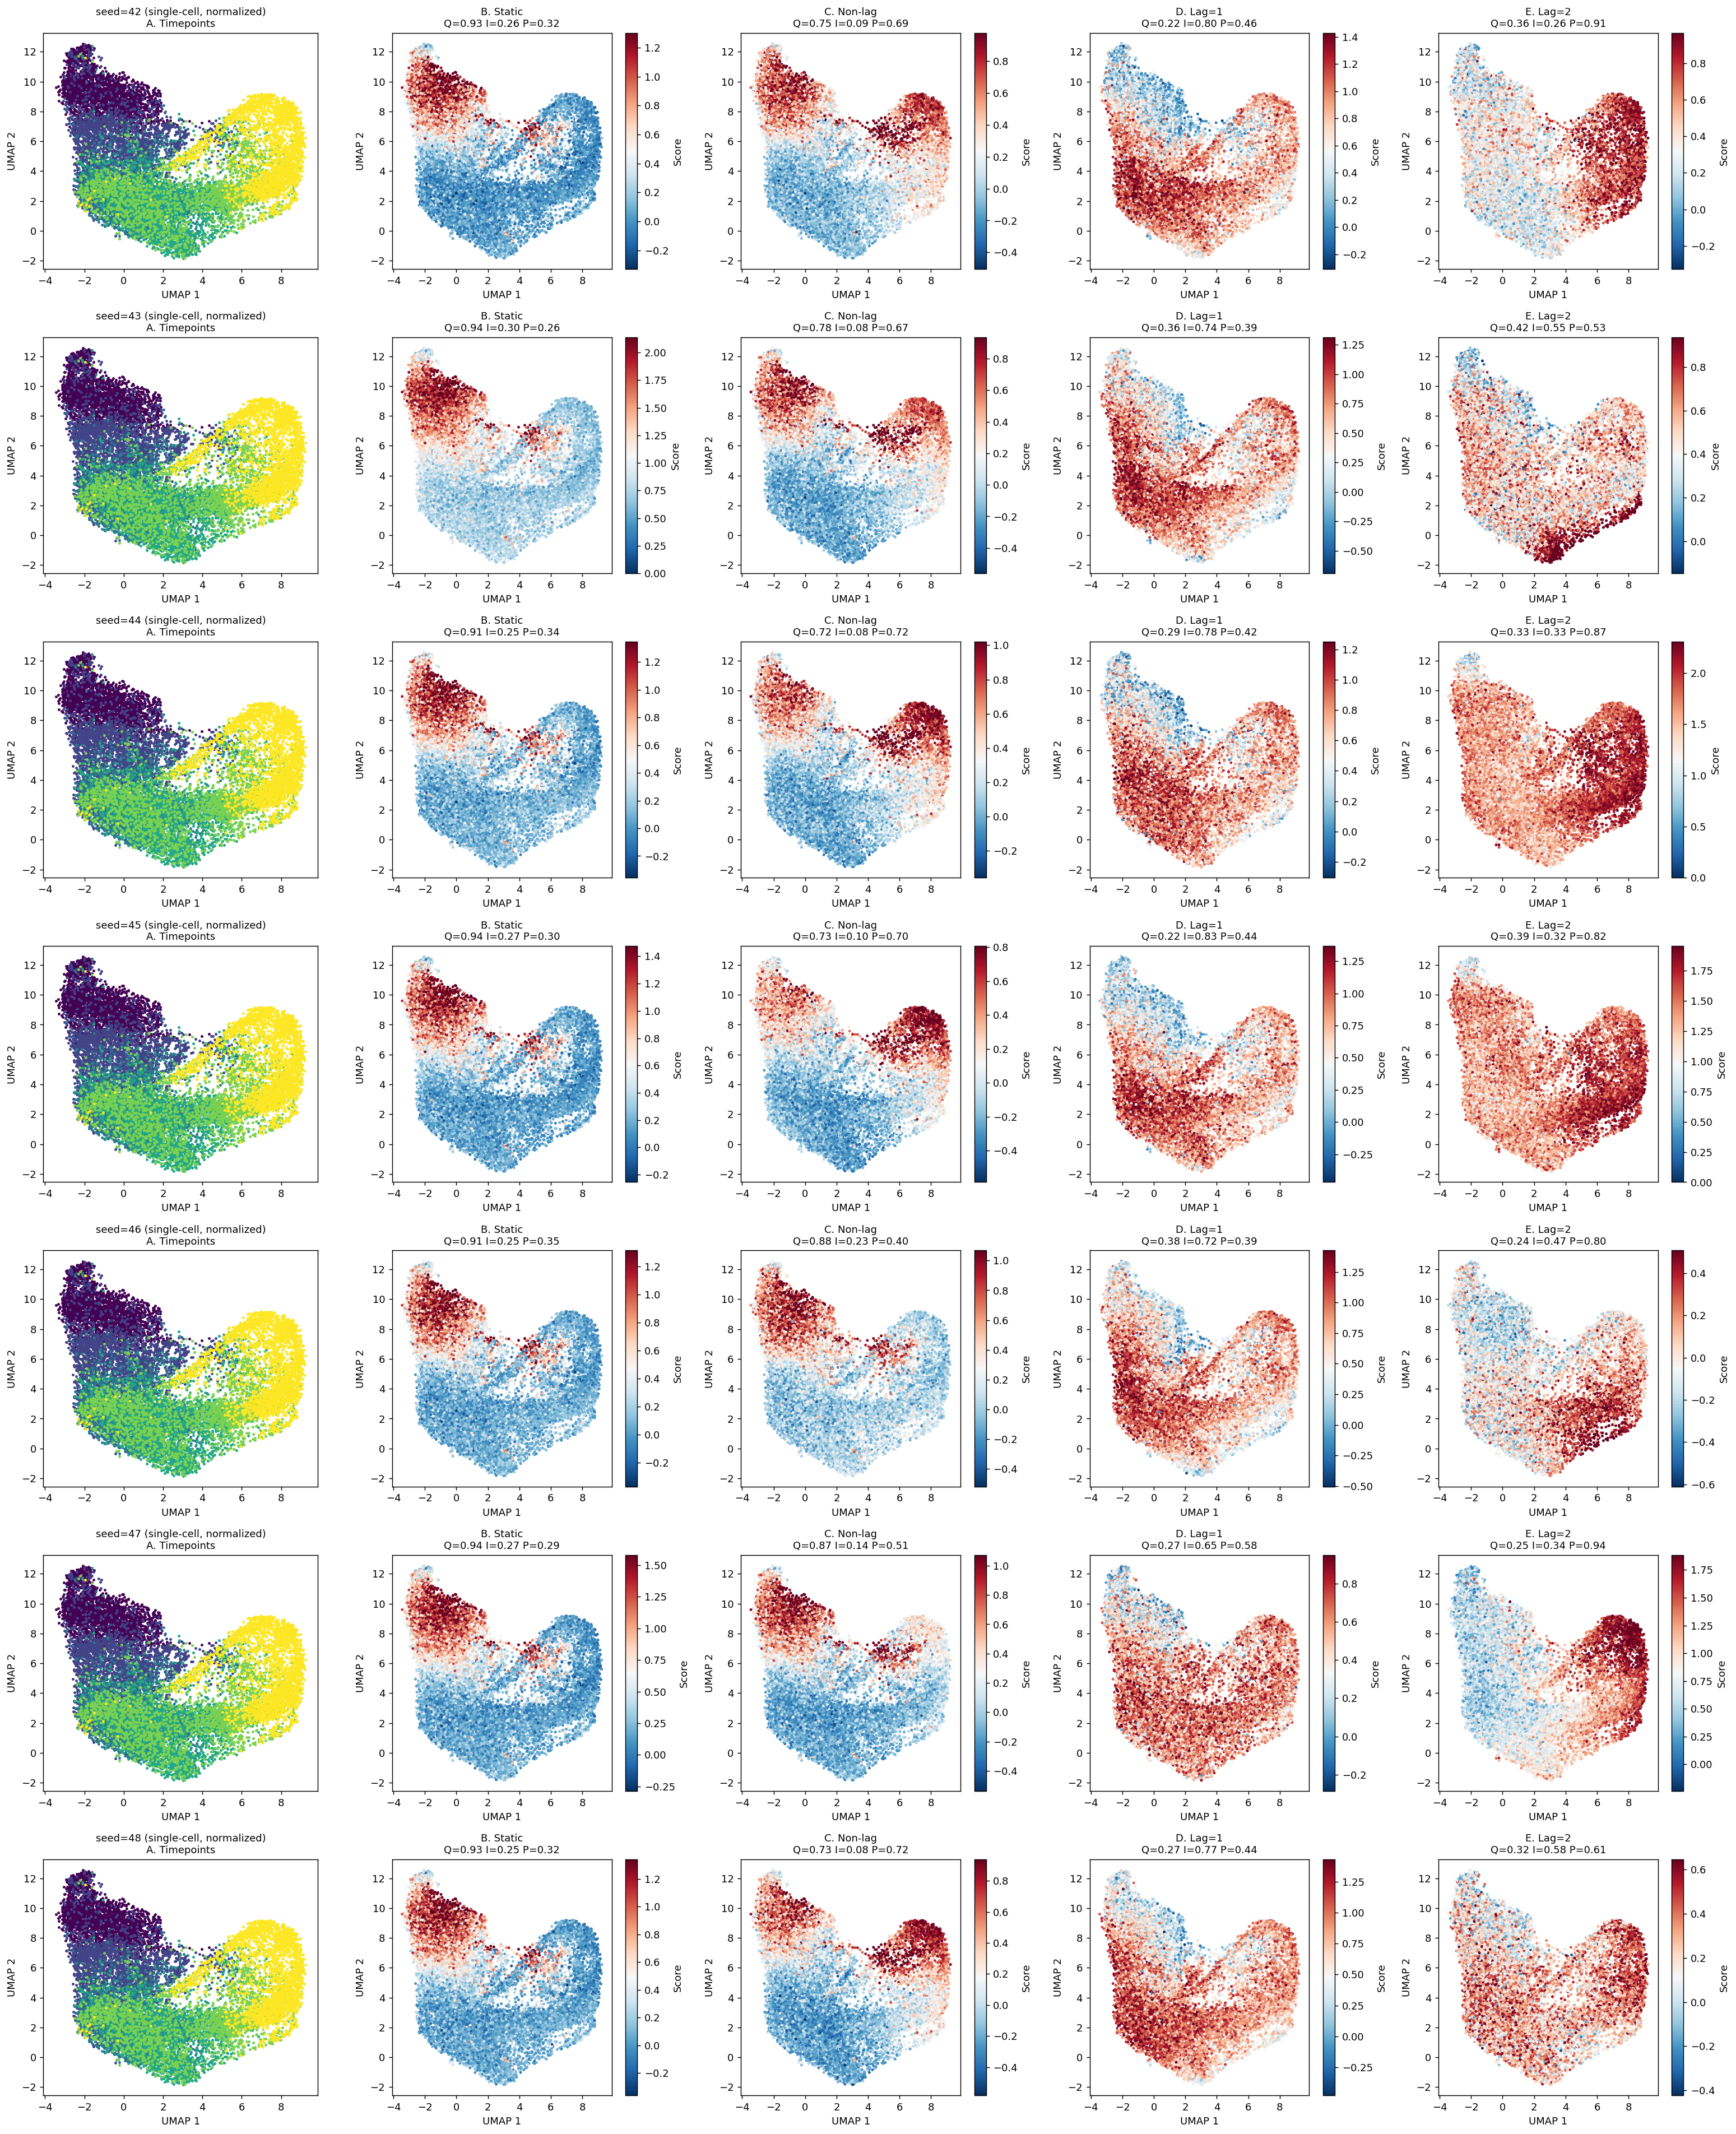
\includegraphics[width=\linewidth]{pictures/rms_multiseed_grid_noPctPos.png}
    \caption{HSPA1B query across 7 GCN/DeepSets training seeds (42--48). Each row shows Timepoints, Static, Non-lag, Lag=1 and Lag=2 program scores for one seed; AUROC (Q/I/P) is reported per panel. The quiescent$\to$intermediate$\to$proliferative shift from Static/Non-lag to Lag=2 is visible in 6 of 7 seeds.}
    \label{fig:multiseed_umap}
\end{figure}


The reciprocal MKI67 query (Fig.~\ref{fig:mki67_panels}) is proliferative-dominant at the first two levels, dips transiently toward intermediate at lag 1 and returns to proliferative at lag 2.

\begin{table}[h]
\centering
\caption{Program-score AUROC by level and seed gene.}
\begin{tabular}{lccc}
\toprule
 & Quiescent & Intermediate & Proliferative \\
\midrule
\multicolumn{4}{l}{\textit{HSPA1B}} \\
Static & \textbf{0.848} & 0.347 & 0.302 \\
Non-lagged co-change & \textbf{0.919} & 0.236 & 0.349 \\
Lag=1 & 0.351 & \textbf{0.731} & 0.404 \\
Lag=2 & 0.418 & 0.143 & \textbf{0.979} \\
\midrule
\multicolumn{4}{l}{\textit{MKI67}} \\
Static & 0.482 & 0.137 & \textbf{0.918} \\
Non-lagged co-change & 0.512 & 0.125 & \textbf{0.900} \\
Lag=1 & 0.261 & \textbf{0.757} & 0.469 \\
Lag=2 & 0.383 & 0.195 & \textbf{0.960} \\
\bottomrule
\end{tabular}
\label{tab:rms-levels-full}
\end{table}

\begin{figure}[h]
    \centering
    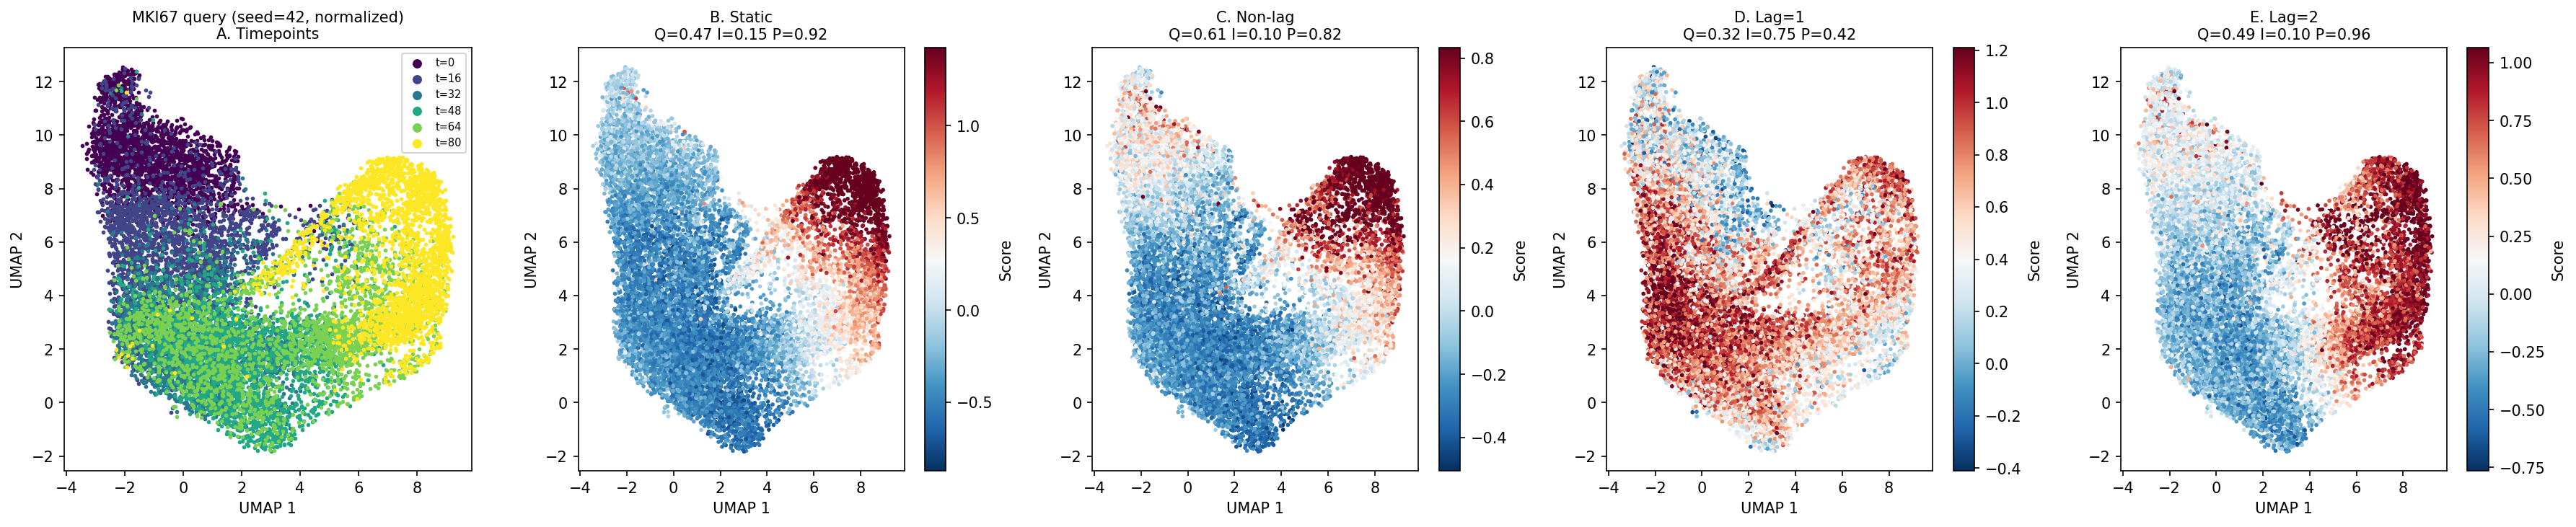
\includegraphics[width=\linewidth]{pictures/rms_normalized_seed42_MKI67.png}
    \caption{MKI67 query, reciprocal to Fig.~\ref{fig:umap_programs}. Static and non-lagged retrieval are already proliferative-dominant; lag 1 transiently loses proliferative specificity in favour of the intermediate compartment, and lag 2 restores it.}
    \label{fig:mki67_panels}
\end{figure}



A core-to-core bridge query gives a further check. We take the top-30 genes by non-lag $\delta_{\mathrm{KL}}$ similarity to HSPA1B and to MKI67 as two cores, and combine them with the max-score formula of \S\ref{sec:bridge} restricted to the lag-2 KL channel. This gives an AUROC of $0.892$ against proliferative for HSPA1B-core$\to$MKI67-core. In the reverse direction, MKI67-core$\to$HSPA1B-core is weak against proliferative ($0.453$) but discriminates the intermediate compartment instead ($0.752$), indicating an asymmetric bridge context associated with the transitional state rather than a simple mirror of the forward direction.


\section{Gene embedding trajectories: full construction}
\label{app:embedding}

\subsection*{Co-expression embedding}

Let $\mathcal{G}=\{g_1,\ldots,g_n\}$ be genes observed at $t_0<\cdots<t_M$. At each timepoint, the Pearson correlation matrix $C_t(i,j)=\operatorname{corr}(x_i^t,x_j^t)$ defines a weighted graph with soft-thresholded weights $A_t\in[0,1]^{n\times n}$~\cite{langfelder2008wgcna}. A GCN~\cite{kipf2017gcn} with weights shared across timepoints takes $H_t^{(0)}=C_t$ and propagates
\[
H_t^{(\ell+1)}=\eta\!\left(D_t^{-1/2}A_tD_t^{-1/2}H_t^{(\ell)}W^{(\ell)}\right),\qquad D_t(i,i)=\sum_jA_t(i,j),
\]
where $\eta$ is the ELU nonlinearity and no additional self-loops are added. The final layer gives $\zco_t(i)=H_t^{(L)}(i,\cdot)\in\mathbb{R}^d$. The encoder is trained as a graph autoencoder~\cite{kipf2016vgae} with a raw inner-product decoder $\widehat{A}_t(i,j)=\zco_t(i)^\top\zco_t(j)$ and loss
\[
\mathcal{L}_{\mathrm{graph}}=\frac{1}{|\mathcal{E}_t|}\sum_{(i,j)\in\mathcal{E}_t}\big(\widehat{A}_t(i,j)-A_t(i,j)\big)^2 .
\]

\subsection*{Marginal-expression embedding}

For gene $i$ at timepoint $t$, let $S_i^t=\{x_{ic}^t\}_{c=1}^{N_t}$ be its library-normalised log-expression values. Values are standardised with a fixed reference, $\widetilde{x}_{ic}^t=(x_{ic}^t-\mu_{\mathrm{ref}})/\sigma_{\mathrm{ref}}$, using the same $\mu_{\mathrm{ref}},\sigma_{\mathrm{ref}}$ for all genes and timepoints. A DeepSets encoder~\cite{zaheer2017deep} maps each value through $h_{ic}^t=\phi_\theta(\widetilde{x}_{ic}^t)$, aggregates $u_i^t=[\operatorname{mean}_c h_{ic}^t\,\Vert\,\operatorname{std}_c h_{ic}^t]$, and outputs $\zex_t(i)=\rho_\theta(u_i^t)\in\mathbb{R}^P$. A decoder $\mathcal{D}_\theta$ reconstructs the empirical quantile vector $Q_i^t=[F_{i,t}^{-1}(q_1),\ldots,F_{i,t}^{-1}(q_{49})]$, with $q_k$ equally spaced in $[0.01,0.99]$, through
\[
\mathcal{L}_{\mathrm{rec}}=\big\|\mathcal{D}_\theta(\zex_t(i))-Q_i^t\big\|_2^2 .
\]
For two independent cell subsamples of the same gene and timepoint, a consistency term penalises differing embeddings:
\[
\mathcal{L}_{\mathrm{cons}}=\big\|f_\theta(S_{i,t}^{(1)})-f_\theta(S_{i,t}^{(2)})\big\|_2^2,\qquad
\mathcal{L}_{\mathrm{expr}}=\mathcal{L}_{\mathrm{rec}}+\lambda_{\mathrm{cons}}\mathcal{L}_{\mathrm{cons}} .
\]



\end{document}